\documentclass{beamer}


\usepackage{amsmath, fontspec}
\usefonttheme{serif}

\usepackage[document]{ragged2e}
\usepackage{xeCJK}
\setCJKmainfont{SimSun} % 设置中文字体为宋体


\usepackage{beamerthemesplit} % 加载主题宏包
\usetheme{Warsaw} % 选用该主题


%插入图片, 写公式, 画表格等
\usepackage{subfig}
\usepackage{amssymb,mathtools}
\usepackage{amsfonts,booktabs}
\usepackage{lmodern,textcomp}
\usepackage{color}
\usepackage{tikz}
\usepackage[utf8]{inputenc}
\usepackage{natbib}
\usepackage{multicol}
\usepackage{graphicx}
\usepackage{bm}

\setbeamertemplate{footline}{\hfill\insertframenumber/\inserttotalframenumber} % 页脚为页码
\setbeamertemplate{headline}{}

%%%%%%%%%%%%%%%%%%%%%%%%%%%%%%%%%%%%%%%%%%%%%%%%%%%%%%%
% 自定义一个输入代码的环境
%\usepackage{listings}
%\usepackage{xcolor}
%%%%%%%%%%%%%%%%%%%%%%%%%%%%%%%%%%%%%%%%%%%%%%%%%%%%%%%%
% 注意这部分代码将全角的逗号句号转换为了半角的逗号句号且半角逗号后面跟了一个空格,要求用xelatex编译,但模板撰写的时候默认用pdflatex,不推荐使用

\catcode`,=\active
\newcommand{,}{, }

\catcode`。=\active
\newcommand{。}{.}

\catcode`:=\active
\newcommand{:}{: }
%%%%%%%%%%%%%%%%%%%%%%%%%%%%%%%%%%%%%%%%%%%%%%%%%%%%%%%%


\begin{document}
	
	%基本信息
	\title{用最简平面二足模型\\近似 Rigid Ramp Walker 模型的理论尝试}
	%\subtitle{电磁学荣誉课讨论}
	\author{林海轩}
	\institute{复旦大学物理学系}
	\date{}
	
	%生成标题页
	\begin{frame}
		\titlepage
	\end{frame}
	
	%目录页,代码无需改动
	\begin{frame}
		\tableofcontents
	\end{frame}
	
	
	%%%%%%%%%%%%%%%%%%%%%%%%%%%%%%%%%%%%%%%%%%%%%%%%%%%%%%%%%%%%%%%%%%%%%%%%%%%%%%%%%%%%%%%%%%%%%%%
	
	\section{前言}
	\begin{frame}[plain,c]
		\begin{center}
			\Huge 前言
		\end{center}
	\end{frame}
	
	\begin{frame}
		\frametitle{二足模型概览}
		\begin{figure}
			\centering
			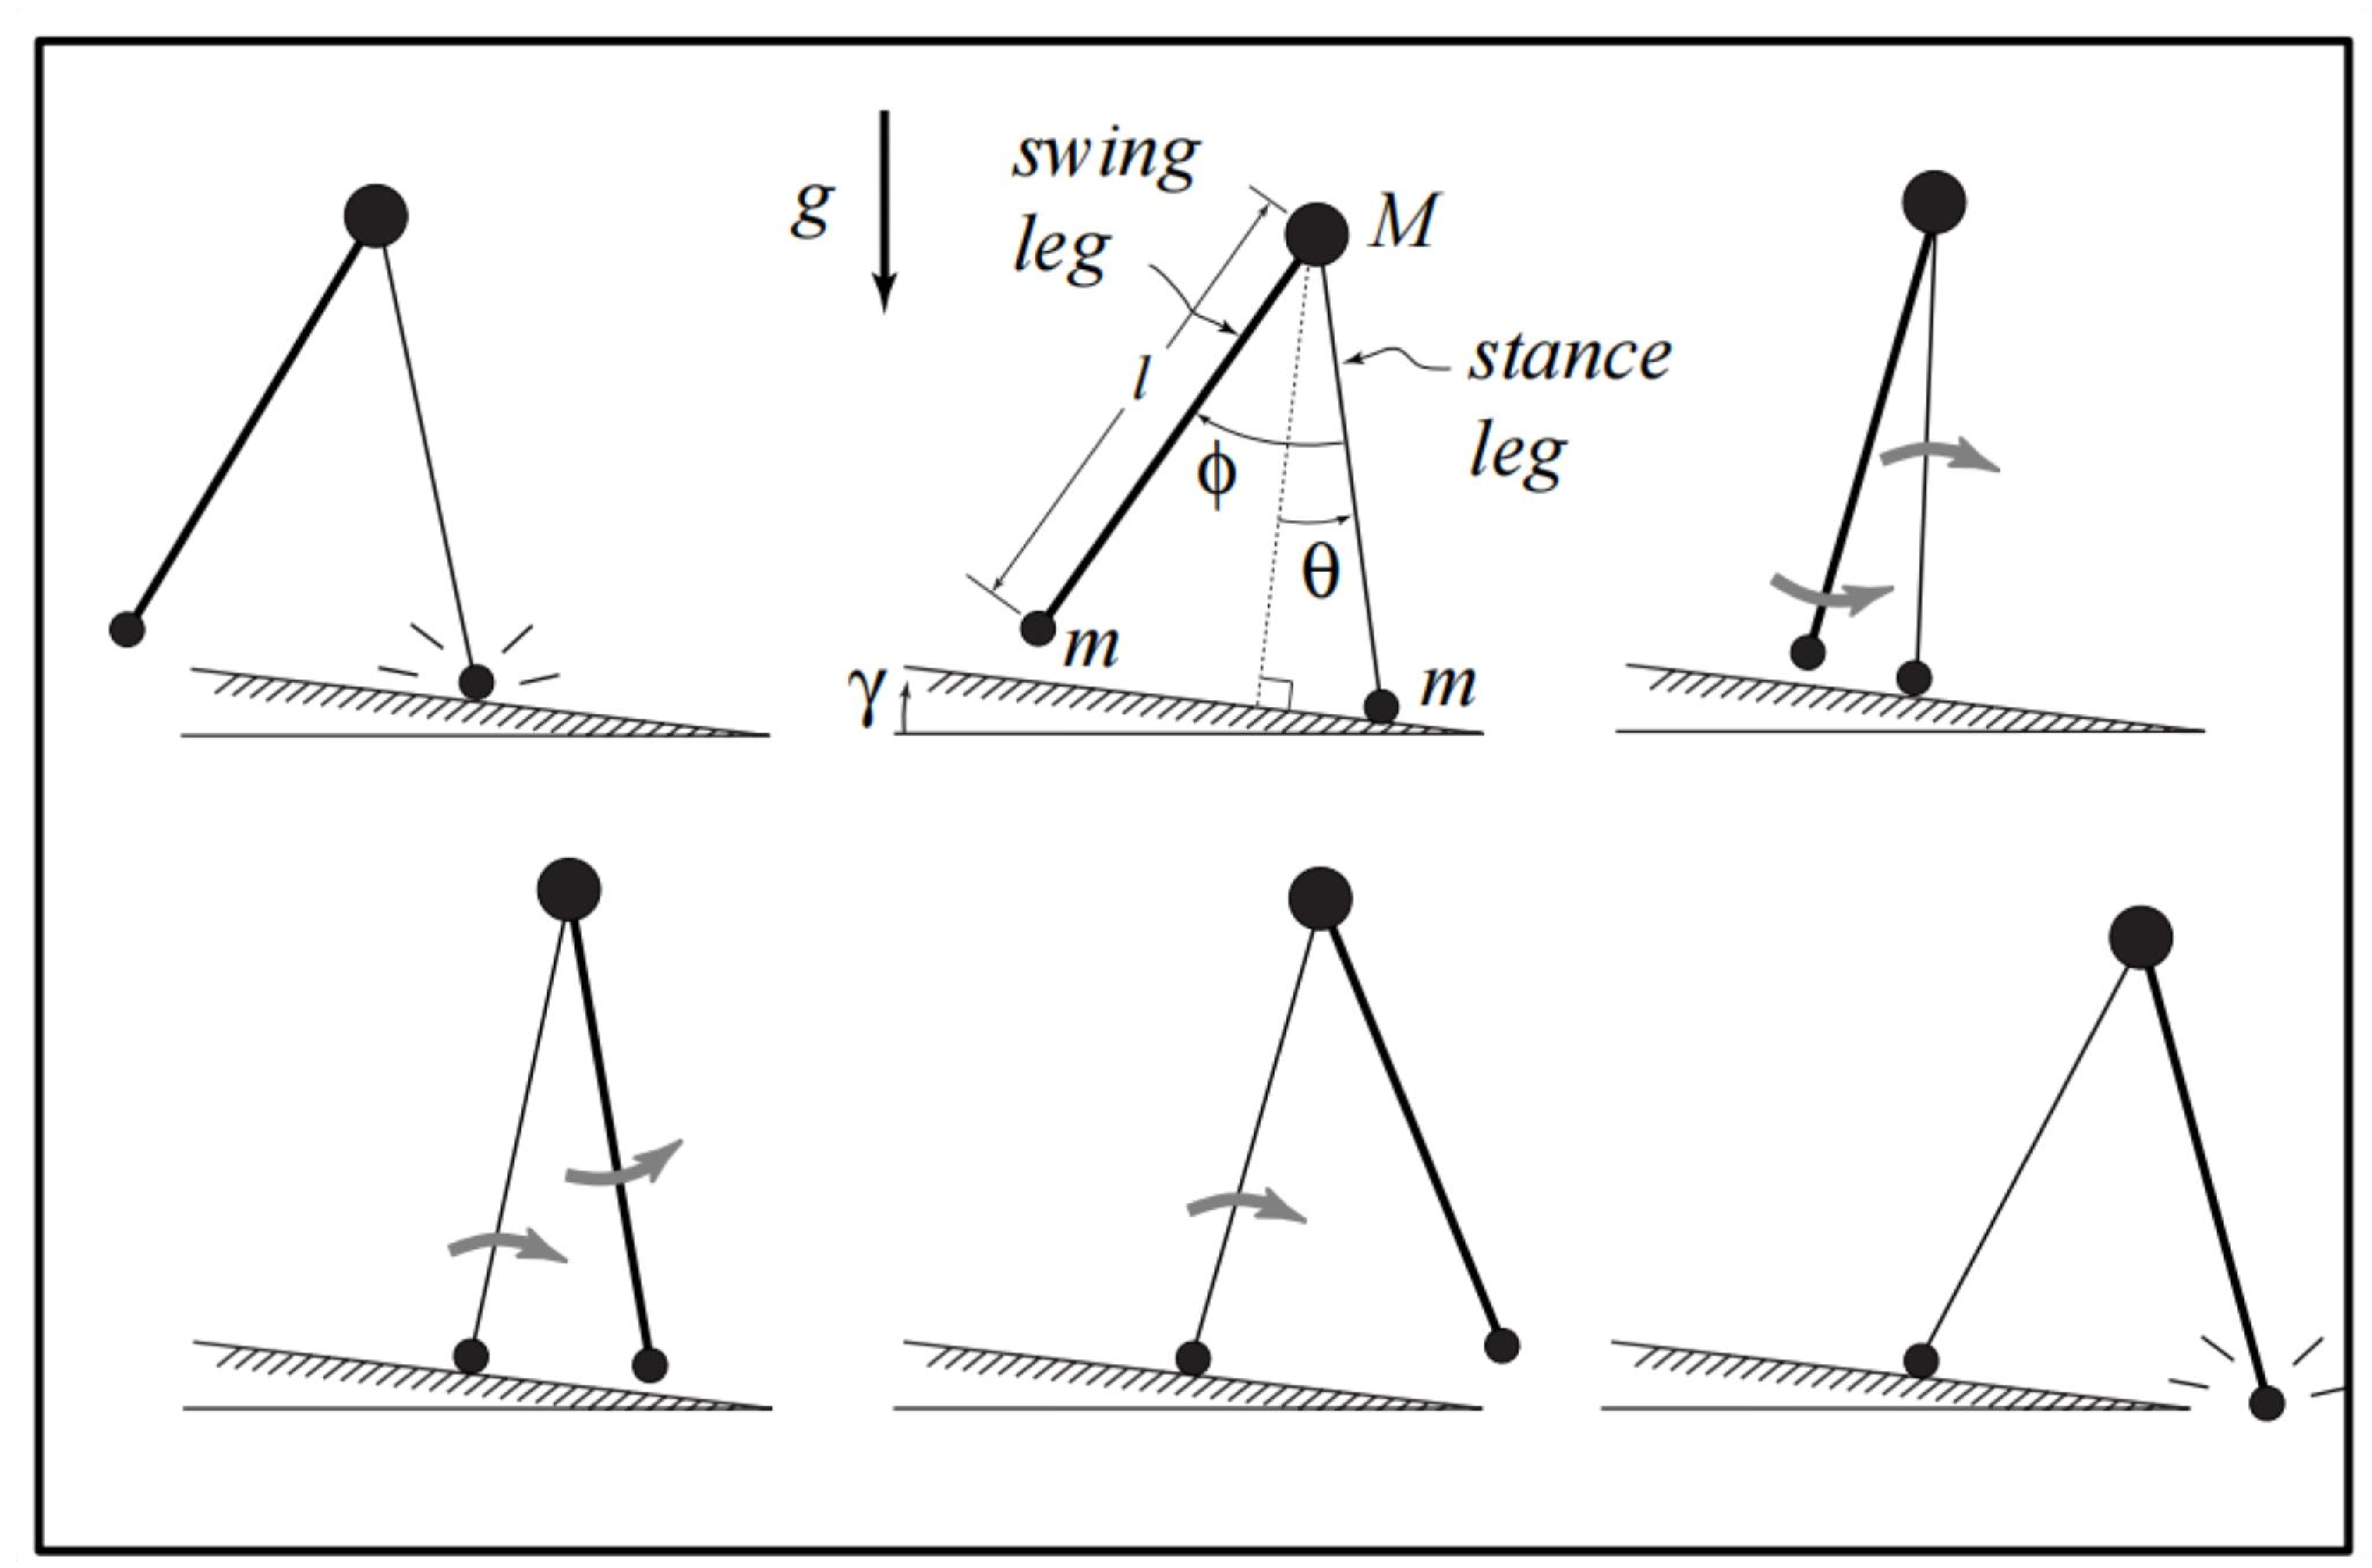
\includegraphics[width=1\linewidth]{McModel}
			\caption*{}
			\label{fig:mcmodel}
		\end{figure}
	\end{frame}
	\begin{frame}
		\frametitle{为什么要研究如此“简单”的模型?}
		相较于完全自创的复杂模型,往已经被前人研究过的简单模型中添加修正后,如果能得到可以解释实验所得的结果,则计算量更小,过程更清晰,结果更令人信服。
	\end{frame}
	
	\begin{frame}
		\frametitle{为什么要研究二足模型而不是四足模型?}
		一方面,根据阅读文献,似乎没有找到四足模型完全理论化的方程。
		
		另一方面,根据我本人最初的想法,这个二足模型通过添加阻尼项,劲度系数项,左右半身耦合项,可以很大程度解释四足的情况,抑或是把最后的结果直接与四足实验数据作差求得两模型的差异,为进一步的研究提供方向。
		
		同时,二足模型的研究方法可以为四足模型的研究提供思路,见另一篇ppt。
	\end{frame}
	
	
	\section{假设、约定与符号}
	
	\begin{frame}[plain,c]
		\begin{center}
			\Huge 假设、约定与符号
		\end{center}
	\end{frame}
	
	\begin{frame}
		\frametitle{卡通视图以及一些假设与符号}
		\begin{minipage}[l]{0.7\linewidth}
			\begin{figure}
				\centering
				\includegraphics[width=1\linewidth]{"TOW LEGS (1)"}
			\end{figure}
		\end{minipage}
		\begin{minipage}{0.3\linewidth}
			{\small
				\begin{itemize}
						%\raggedright
					\item 刚体假设:\\顶部用一个小球代表身体,底部用两个小球代表足,足和身体之间用相同长度的刚体杆连接
					\item 站立(stance)足与摆动(swift)足约定:\\用细直线代表与地面接触的足,用加粗直线代表正在摆动的足
					\item 理想关节与掠滑过假设:\\关节是无阻尼无恢复系数的,摆动足滑过地面的时候视为无摩擦
				\end{itemize}
			
			}
		\end{minipage}
	\end{frame}
	
	\begin{frame}
		\begin{minipage}[l]{0.7\linewidth}
			\begin{figure}
				\centering
				\includegraphics[width=1\linewidth]{"TOW LEGS (2)"}
			\end{figure}
		\end{minipage}
		\begin{minipage}{0.3\linewidth}
			过身体做一条斜面的垂线,设斜面倾斜角是 $\gamma.$
		\end{minipage}
	\end{frame}
	
	\begin{frame}
		\begin{minipage}[l]{0.7\linewidth}
			\begin{figure}
				\centering
				\includegraphics[width=1\linewidth]{"TOW LEGS (3)"}
			\end{figure}
		\end{minipage}
		\begin{minipage}{0.3\linewidth}
			如图设定两个角参数
		\end{minipage}
	\end{frame}
	
	\begin{frame}
		\begin{minipage}[l]{0.7\linewidth}
			\begin{figure}
				\centering
				\includegraphics[width=1\linewidth]{"TOW LEGS (4)"}
			\end{figure}
		\end{minipage}
		\begin{minipage}{0.3\linewidth}
			设腿长为 $l$,足质量为 $m$,身体质量为 $M$,且 $$\displaystyle \beta=\dfrac{m}{M}$$
		\end{minipage}
	\end{frame}
	
	\section{方程推导}
	\begin{frame}[plain,c]
		\begin{center}
			\Huge 方程推导
		\end{center}
	\end{frame}
	\begin{frame}
		\frametitle{Euler-Lagrange 方程}
		设 $\mathcal{L}=\mathcal{L}(q,\dot{q},t)$ 是Lagrange量, 其中 $q$ 是广义坐标, 运算 $\dot{x}=\dfrac{\mathrm{d}x}{\mathrm{d}t}$表示对时间求一次导数, $\displaystyle S[q]=\int_{t_1}^{t_2}\hspace{-5pt}\mathcal{L}\mathrm{d}t$ 是作用量, 当作用量取得极值($\delta S=0$)时, 有
		\begin{equation}
			\frac{\mathrm{d}}{\mathrm{d}t}\frac{\partial \mathcal{L}}{\partial \dot{q}_i}-\frac{\partial \mathcal{L}}{\partial q_i}=0\nonumber
		\end{equation}
		我们要考察的是连杆模型,显然,杆的端点的力是不好分析的,采用此方程能更方便地描述系统.
	\end{frame}

	\begin{frame}
		\frametitle{势能}
		\begin{figure}
			\centering
			\includegraphics[width=0.7\linewidth]{"TOW LEGS (5)"}
			\label{fig:tow-legs-5}
		\end{figure}
		以站立足为势能零点,可以写出系统的势能
		$$
		V=Mgl\cos \left( \theta -\gamma \right) +mgl\left( \cos \left( \theta -\gamma \right) -\cos \left( \phi -\theta +\gamma \right) \right) 
		$$
	\end{frame}
		
	\begin{frame}
		\frametitle{动能}
		\begin{figure}
			\centering
			\includegraphics[width=0.7\linewidth]{"TOW LEGS (6)"}
			\label{fig:tow-legs-6}
		\end{figure}
		写出身体与摆动足的坐标
		$$
		\bm{M}=\left( \begin{array}{c}
			-l\sin \theta\\
			\hphantom{-}l\cos \theta\\
		\end{array} \right) \qquad \bm{m}=\left( \begin{array}{c}
			-l\left( \sin \theta +\sin \left( \phi -\theta \right) \right)\\
			\hphantom{-}l\left( \cos \theta -\cos \left( \phi -\theta \right) \right)\\
		\end{array} \right) 
		$$
	\end{frame}
	\begin{frame}
		对坐标求导取模长就得到了速率
		$$
		v_M=l\dot{\theta}\qquad v_m=l\sqrt{\dot{\theta}^2+\left( \dot{\phi}-\dot{\theta} \right) ^2+\cos \phi \left( \dot{\phi}-\dot{\theta} \right)}
		$$
		得到 Lagrange 量
		$$
		\mathcal{L} =T-V=\frac{1}{2}mv_{m}^{2}+\frac{1}{2}Mv_{M}^{2}-V
		$$
		代入关于两个广义坐标的 Euler-Lagrange 方程
		$$
		\left( \begin{array}{c}
			\dfrac{\mathrm{d}}{\mathrm{d}t}\dfrac{\partial}{\partial \dot{\theta}}-\dfrac{\partial}{\partial \theta}
			\\\\
			\dfrac{\mathrm{d}}{\mathrm{d}t}\dfrac{\partial}{\partial \dot{\phi}}-\dfrac{\partial}{\partial \phi}
			\\
		\end{array} \right) \mathcal{L} =0
		$$
		写开来得到
	\end{frame}
	
	\begin{frame}
		\begin{align*}
			&\hphantom{+}
			\left( \begin{matrix}
				1+2\beta \left( 1-\cos \phi \right)&		-\beta \left( 1-\cos \phi \right)\\
				\beta \left( 1-\cos \phi \right)&		-\beta\\
			\end{matrix} \right) \left( \begin{array}{c}
				\ddot{\theta}\\
				\ddot{\phi}\\
			\end{array} \right) \\&+\left( \begin{array}{c}
				-\beta \sin \phi \left( \dot{\phi}^2-2\dot{\theta}\dot{\phi} \right)\\
				\beta \dot{\theta}\sin \phi\\
			\end{array} \right) \\&+\left( \begin{array}{c}
				\frac{\beta g}{l}\left[ \sin \left( \theta -\phi -\gamma \right) -\sin \left( \theta -\gamma \right) \right] -\frac{g}{l}\sin \left( \theta -\gamma \right)\\
				\frac{\beta g}{l}\sin \left( \theta -\phi -\gamma \right)\\
			\end{array} \right) =0
		\end{align*}
	\end{frame}
	
	\begin{frame}
		\begin{figure}
			\centering
			\includegraphics[width=1\linewidth]{"TOW LEGS (8)"}
		\end{figure}
		回顾一个基础的假设:摆动足会无摩擦地滑过斜面
	\end{frame}
	\begin{frame}
		\begin{figure}
			\centering
			\includegraphics[width=0.7\linewidth]{"TOW LEGS (7)"}
		\end{figure}
		
		考虑到脚触地,两个足的定义相交换,'+'表示触地后,'-'表示触地前,当 $\phi-2\theta=0$ 时,$\theta$ 反号.
		
	\end{frame}
	
	\begin{frame}
		$$
		\left( \begin{array}{c}
			\theta\\
			\dot{\theta}\\
			\phi\\
			\dot{\phi}\\
		\end{array} \right) ^+=\left( \begin{matrix}
			-1&		0&		0&		0\\
			0&		\cos 2\theta&		0&		0\\
			-2&		0&		0&		0\\
			0&		\cos 2\theta \left( 1-\cos 2\theta \right)&		0&		0\\
		\end{matrix} \right) ^-\left( \begin{array}{c}
			\theta\\
			\dot{\theta}\\
			\phi\\
			\dot{\phi}\\
		\end{array} \right) ^-
		$$
		
		不考虑定义互换
		$$
		\left( \begin{array}{c}
			\theta\\
			\dot{\theta}\\
			\phi\\
			\dot{\phi}\\
		\end{array} \right) ^+=\left( \begin{matrix}
			1&		0&		0&		0\\
			0&		\cos ^22\theta&		0&		0\\
			2&		0&		0&		0\\
			0&		-\cos 2\theta \left( 1-\cos 2\theta \right)&		0&		0\\
		\end{matrix} \right) ^-\left( \begin{array}{c}
			\theta\\
			\dot{\theta}\\
			\phi\\
			\dot{\phi}\\
		\end{array} \right) ^-
		$$
	\end{frame}
	
	\begin{frame}
		\frametitle{模型的数值解图像}
		\begin{figure}
			\centering
			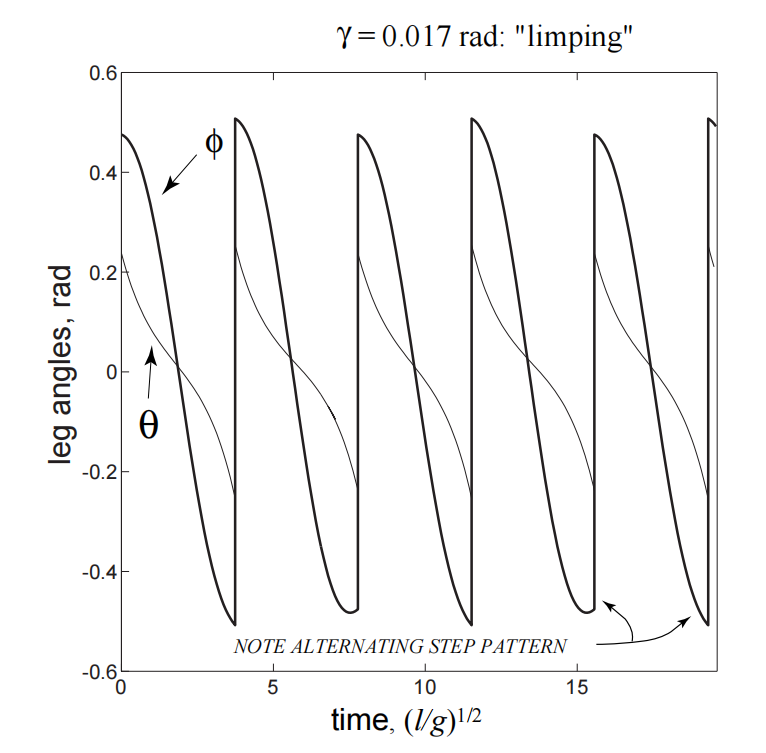
\includegraphics[width=0.8\linewidth]{SolveFromPaper}
			\caption*{}
			\label{fig:solvefrompaper}
		\end{figure}
	\end{frame}
	
	\section{Python代码实现}
	\begin{frame}[plain,c]
		\begin{center}
			\Huge Python代码实现
		\end{center}
	\end{frame}
	\begin{frame}
		\frametitle{Python库}
		\begin{figure}
			\centering
			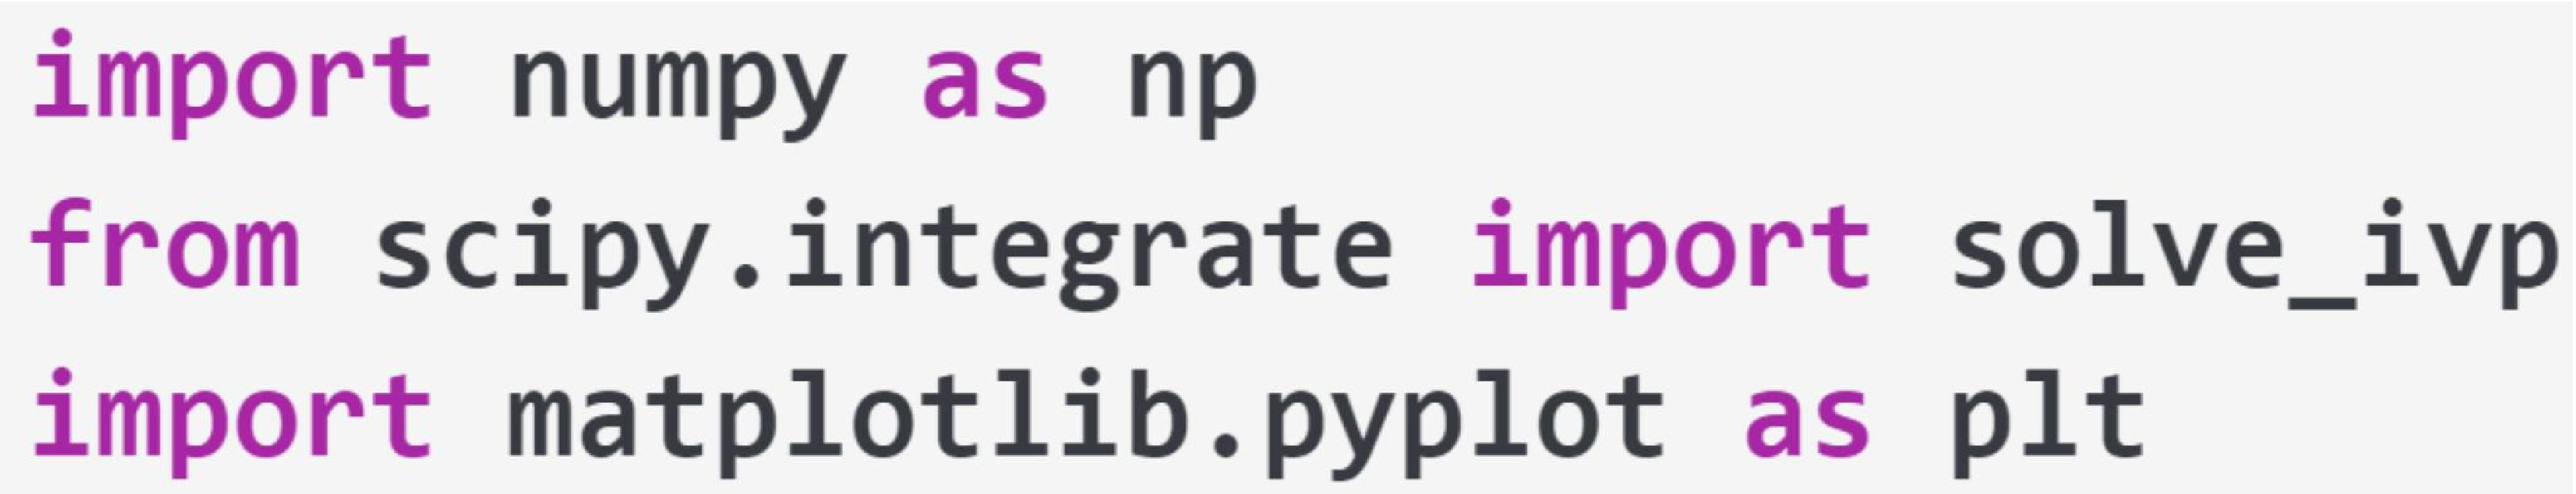
\includegraphics[width=1.0\linewidth]{ModelInPython}
			\caption*{}
			\label{fig:modelinpython}
		\end{figure}
		\begin{enumerate}
			\item numpy库提供了数学里的基本函数,矩阵运算等
			\item solve\_ivp是一个常微分方程求解器,相比于其他求解器它有2个优点: 
			\\
			1. solve\_ivp可以求解刚性微分方程,即允许出现突变的地方 
			\\
			2. solve\_ivp有监测事件的功能,当沿着时间序列对微分方程积分的时候,如果事件函数取得了零点,则可以触发一次事件,对相应的量进行突变调整或改变需要被积分的微分方程,在本情形中对应摆动腿触地(地有瞬时冲量),即一次步态的结束,对应的方程是两只脚定义的呼唤
			\item matplotlib库用以画图,将求得的数值解化为图像验收
		\end{enumerate}
	\end{frame}
	
	\begin{frame}
		\frametitle{通过简单微分方程$\displaystyle \dot{x}=kt$来实践solve\_ivp求解器}
		\begin{figure}
			\centering
			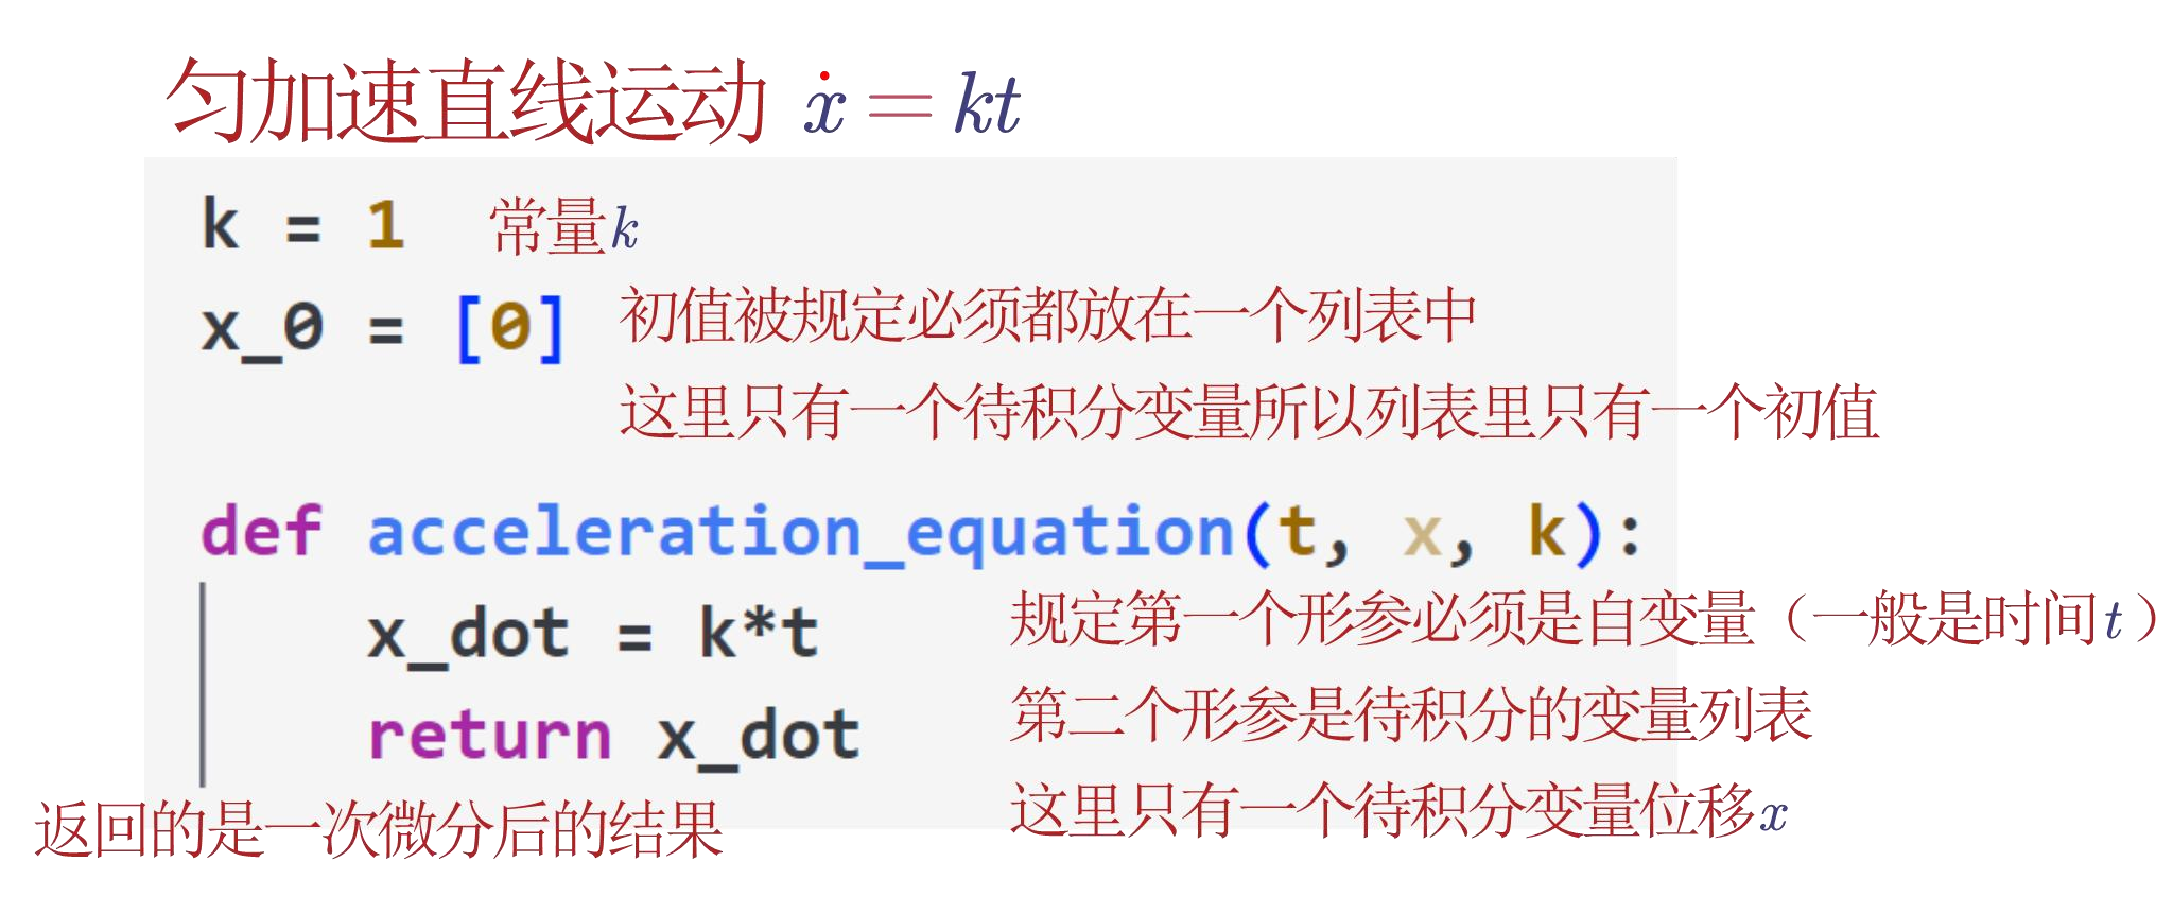
\includegraphics[width=1.1\linewidth]{EasySolve_ivpTourial1}
			\caption*{}
			\label{fig:easysolveivptourial1}
		\end{figure}
	\end{frame}
	
	\begin{frame}
		\begin{figure}
			\centering
			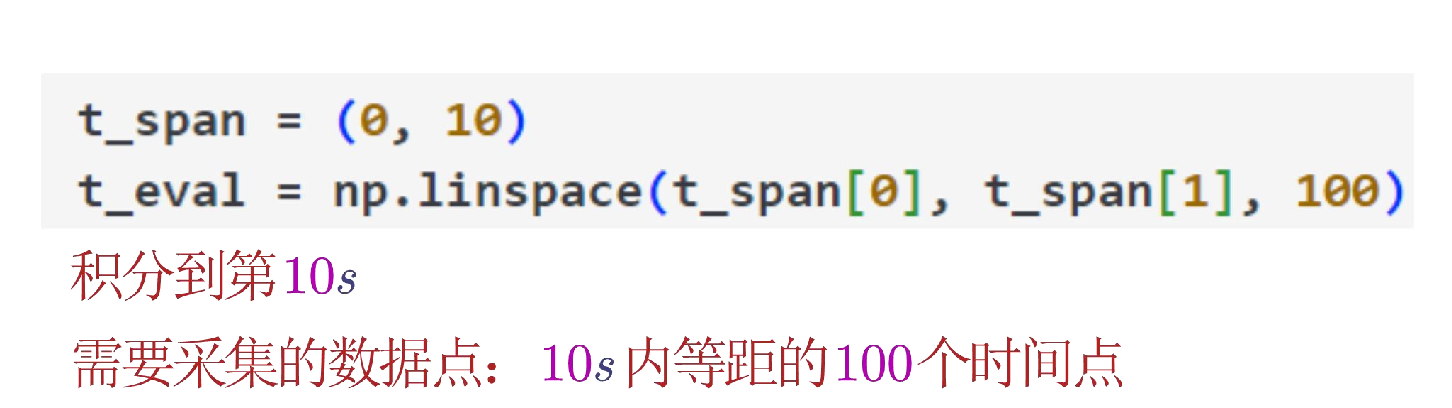
\includegraphics[width=1.1\linewidth]{EasySolve_ivpTourial2}
			\caption*{}
			\label{fig:easysolveivptourial2}
		\end{figure}
	\end{frame}
	
	\begin{frame}
		\begin{figure}
			\centering
			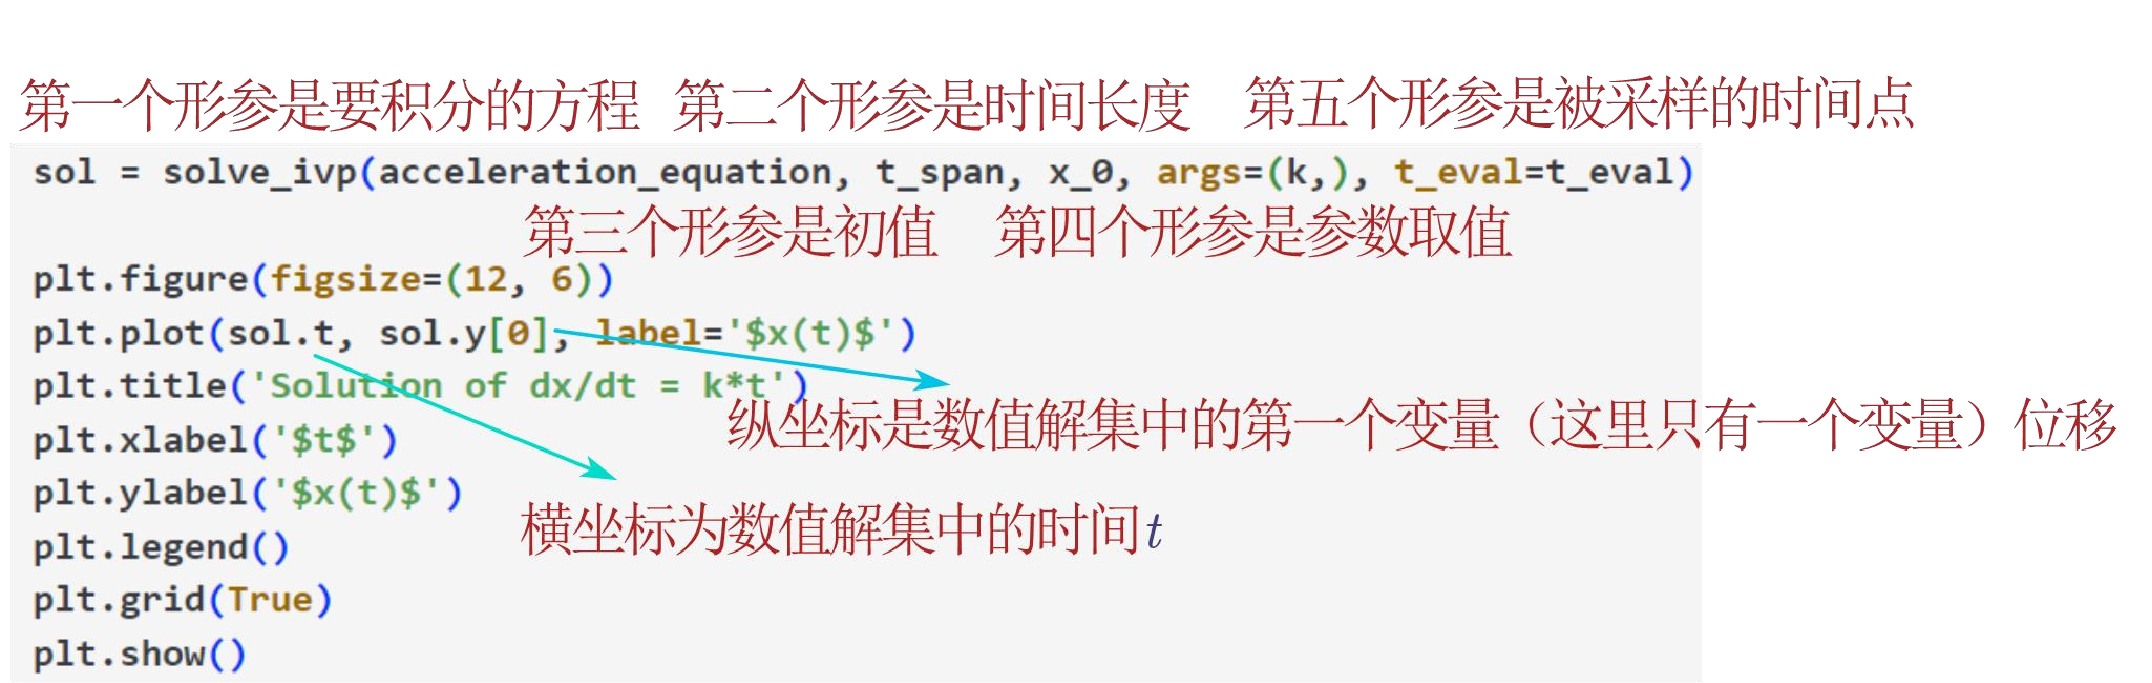
\includegraphics[width=1.1\linewidth]{EasySolve_ivpTourial3}
			\caption*{}
			\label{fig:easysolveivptourial3}
		\end{figure}
	\end{frame}
	
	\begin{frame}
		\begin{figure}
			\centering
			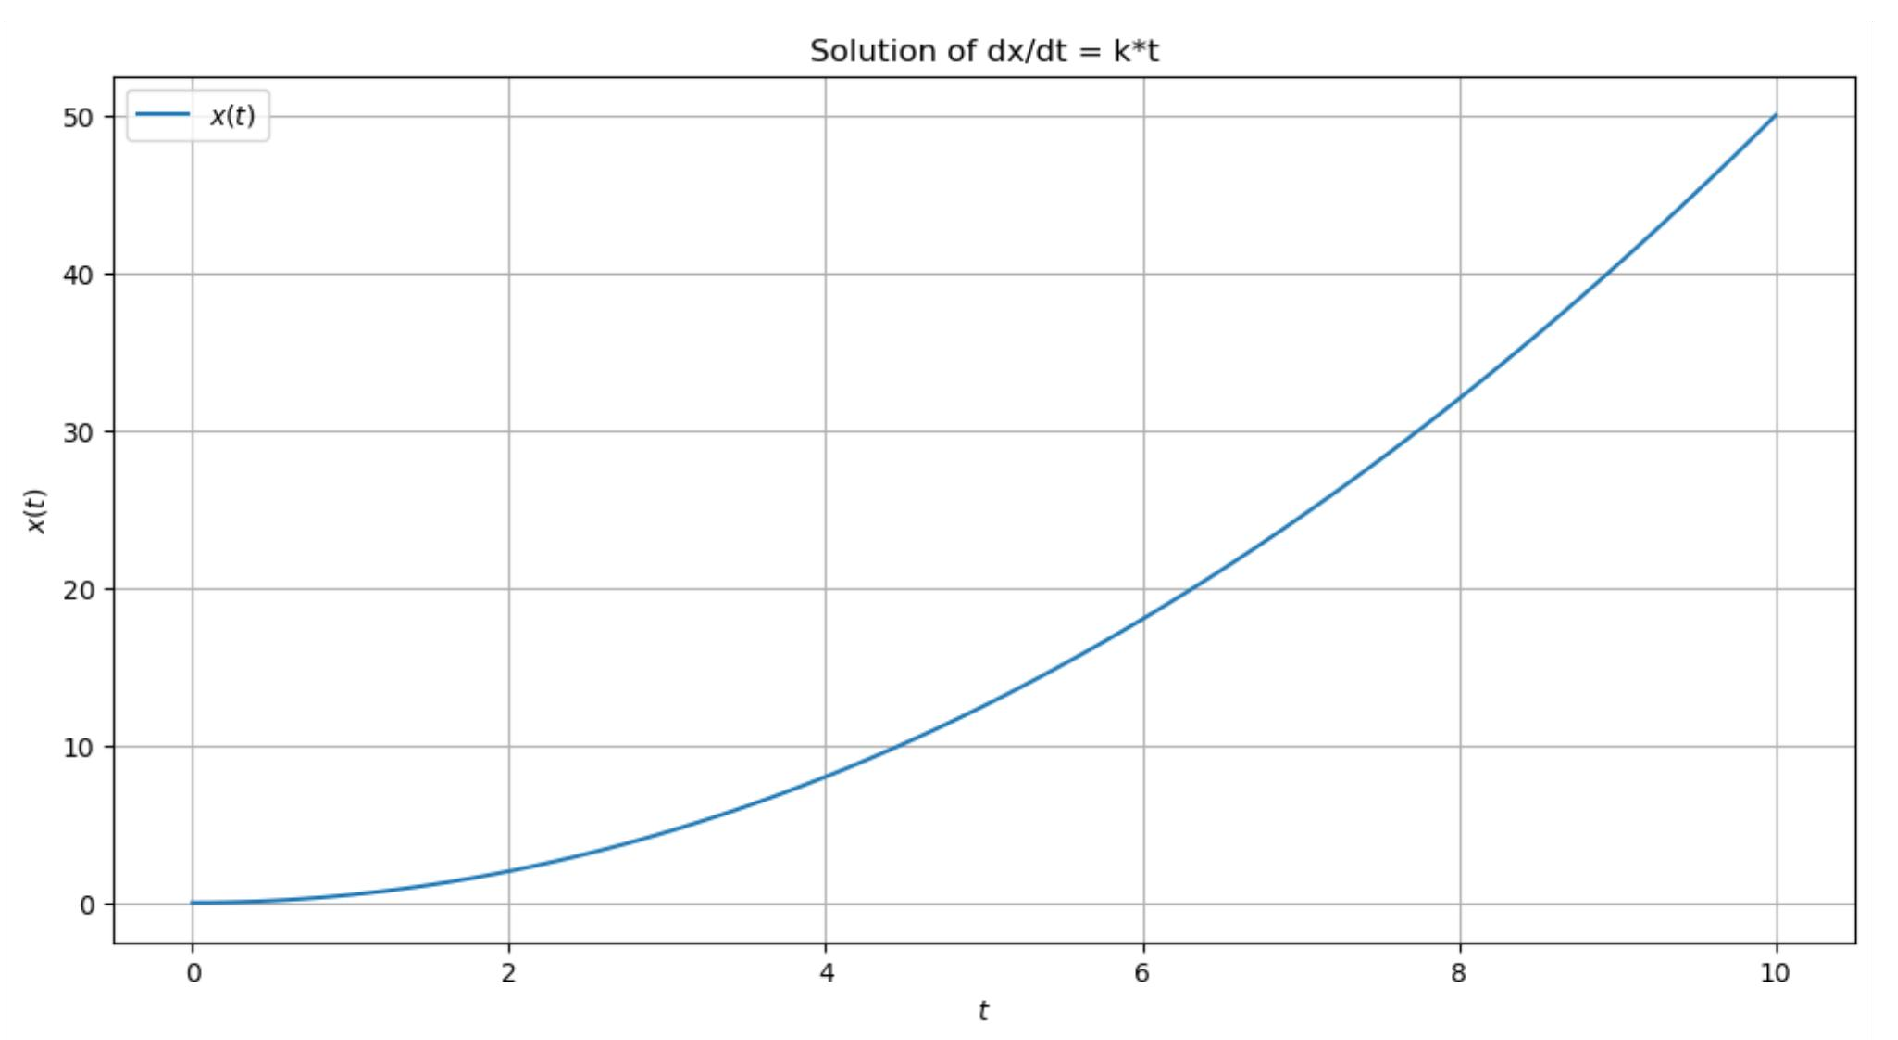
\includegraphics[width=1.1\linewidth]{EasySolve_ivpTourial4}
			\caption*{}
			\label{fig:easysolveivptourial4}
		\end{figure}
	\end{frame}
	
	\begin{frame}
		\frametitle{定义常量和初始化条件}
		下面通过代码来模拟二足模型
		\begin{figure}
			\centering
			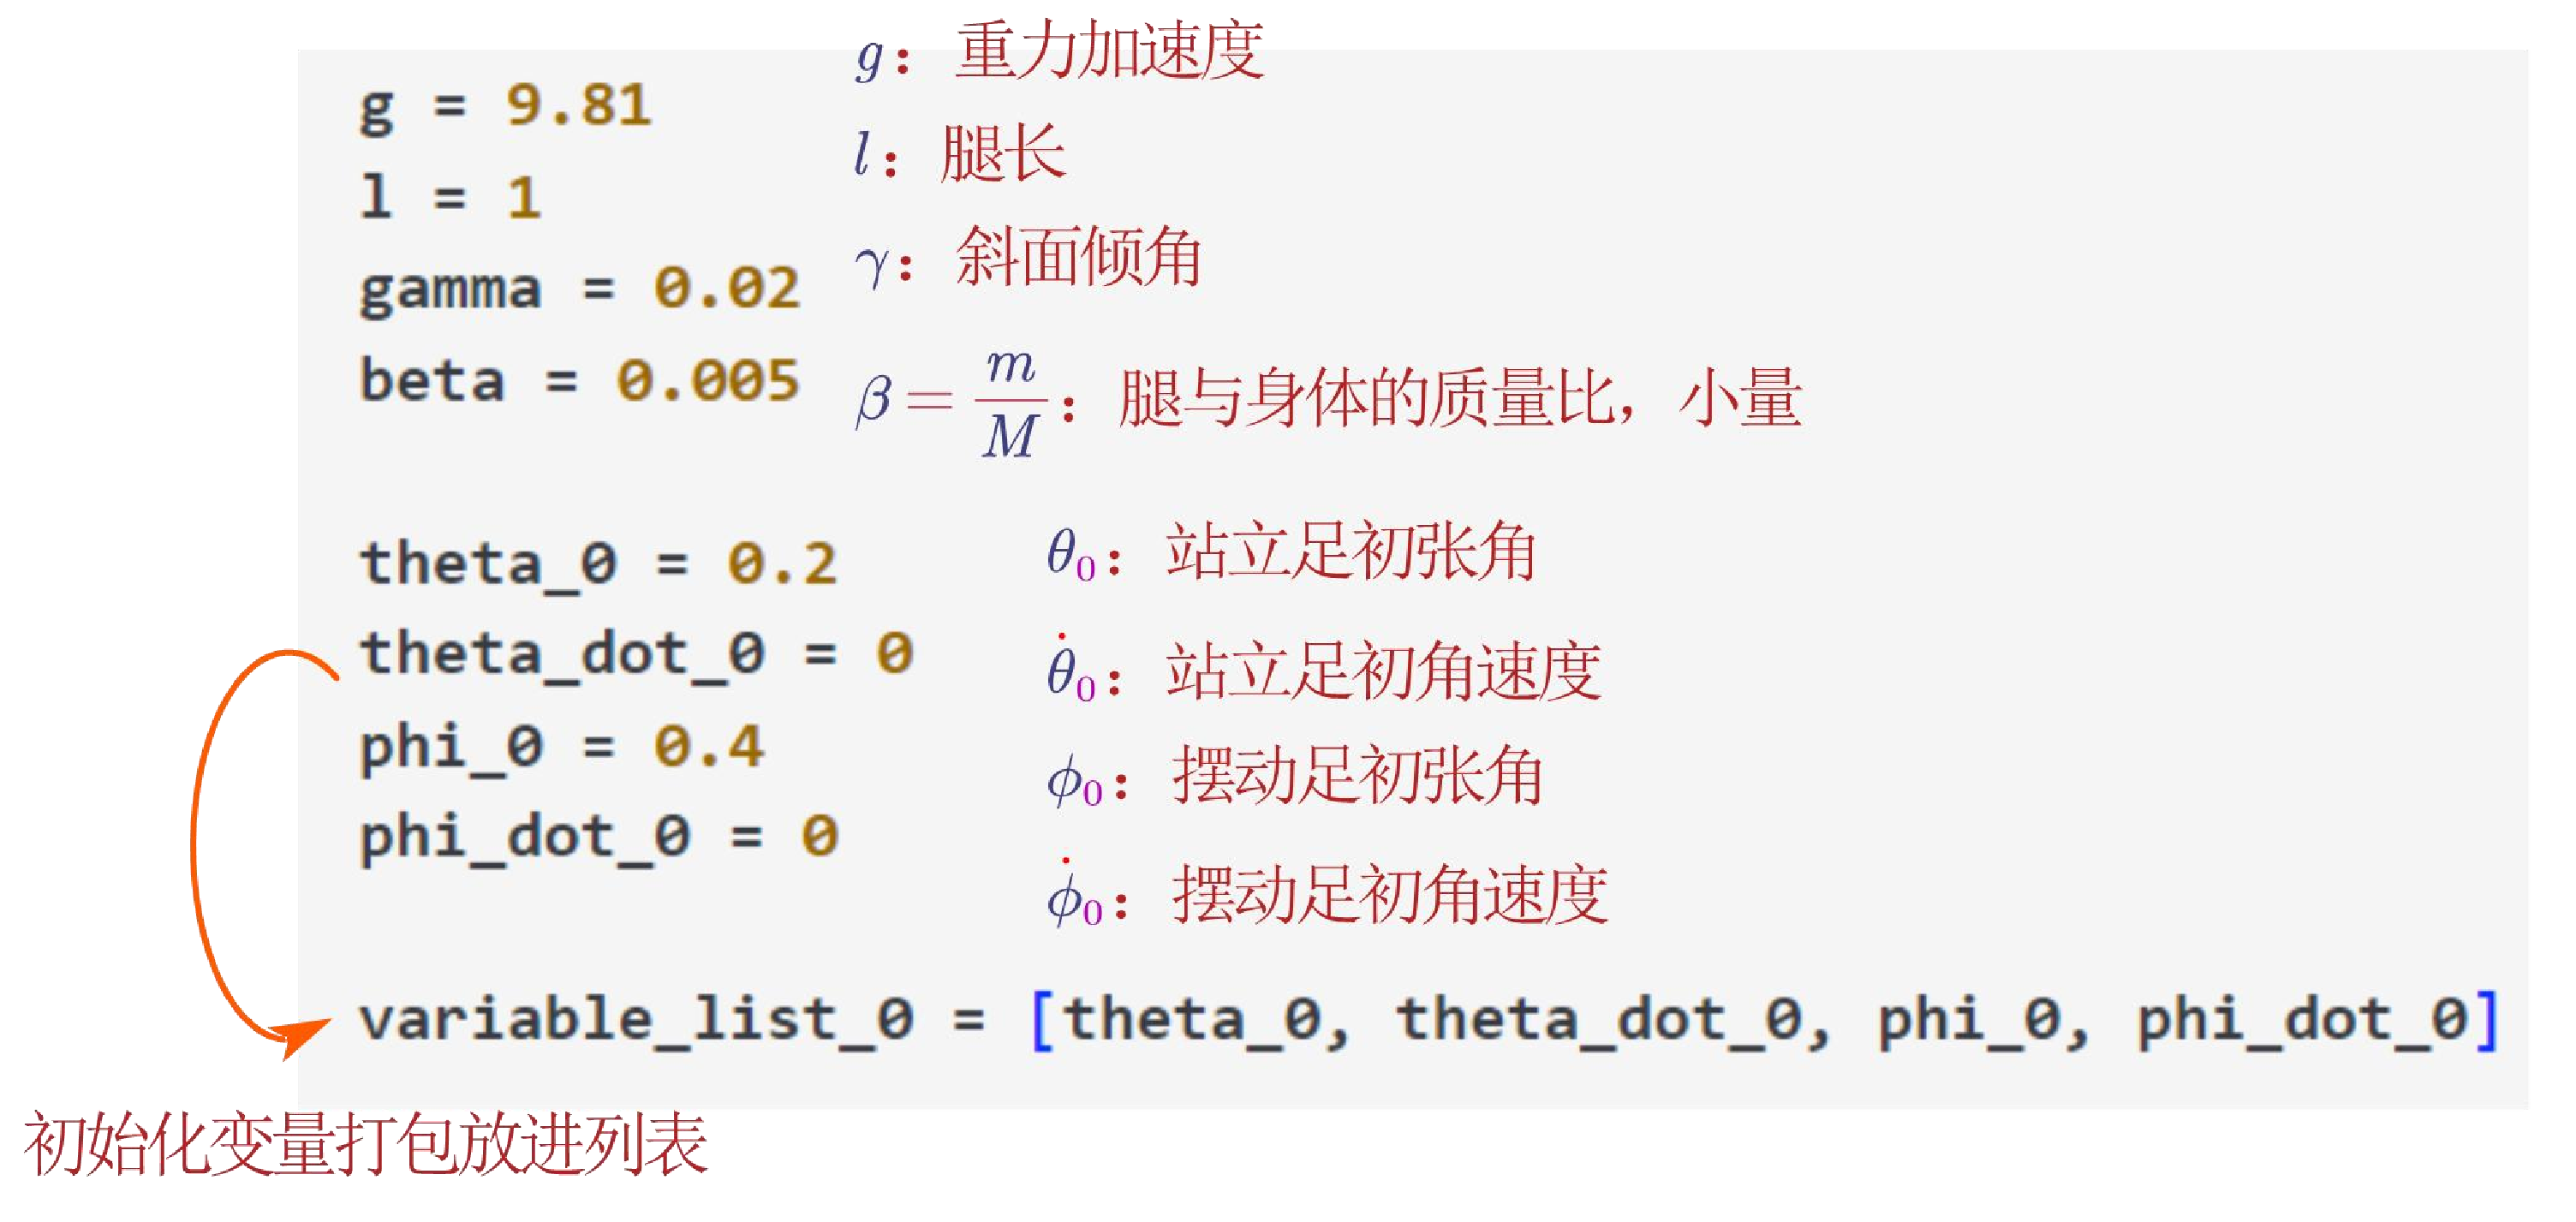
\includegraphics[width=1.1\linewidth]{Initialize}
			\caption*{}
			\label{fig:initialize}
		\end{figure}
	\end{frame}
	
	\begin{frame}
		\frametitle{方程主体}
		\begin{figure}
			\centering
			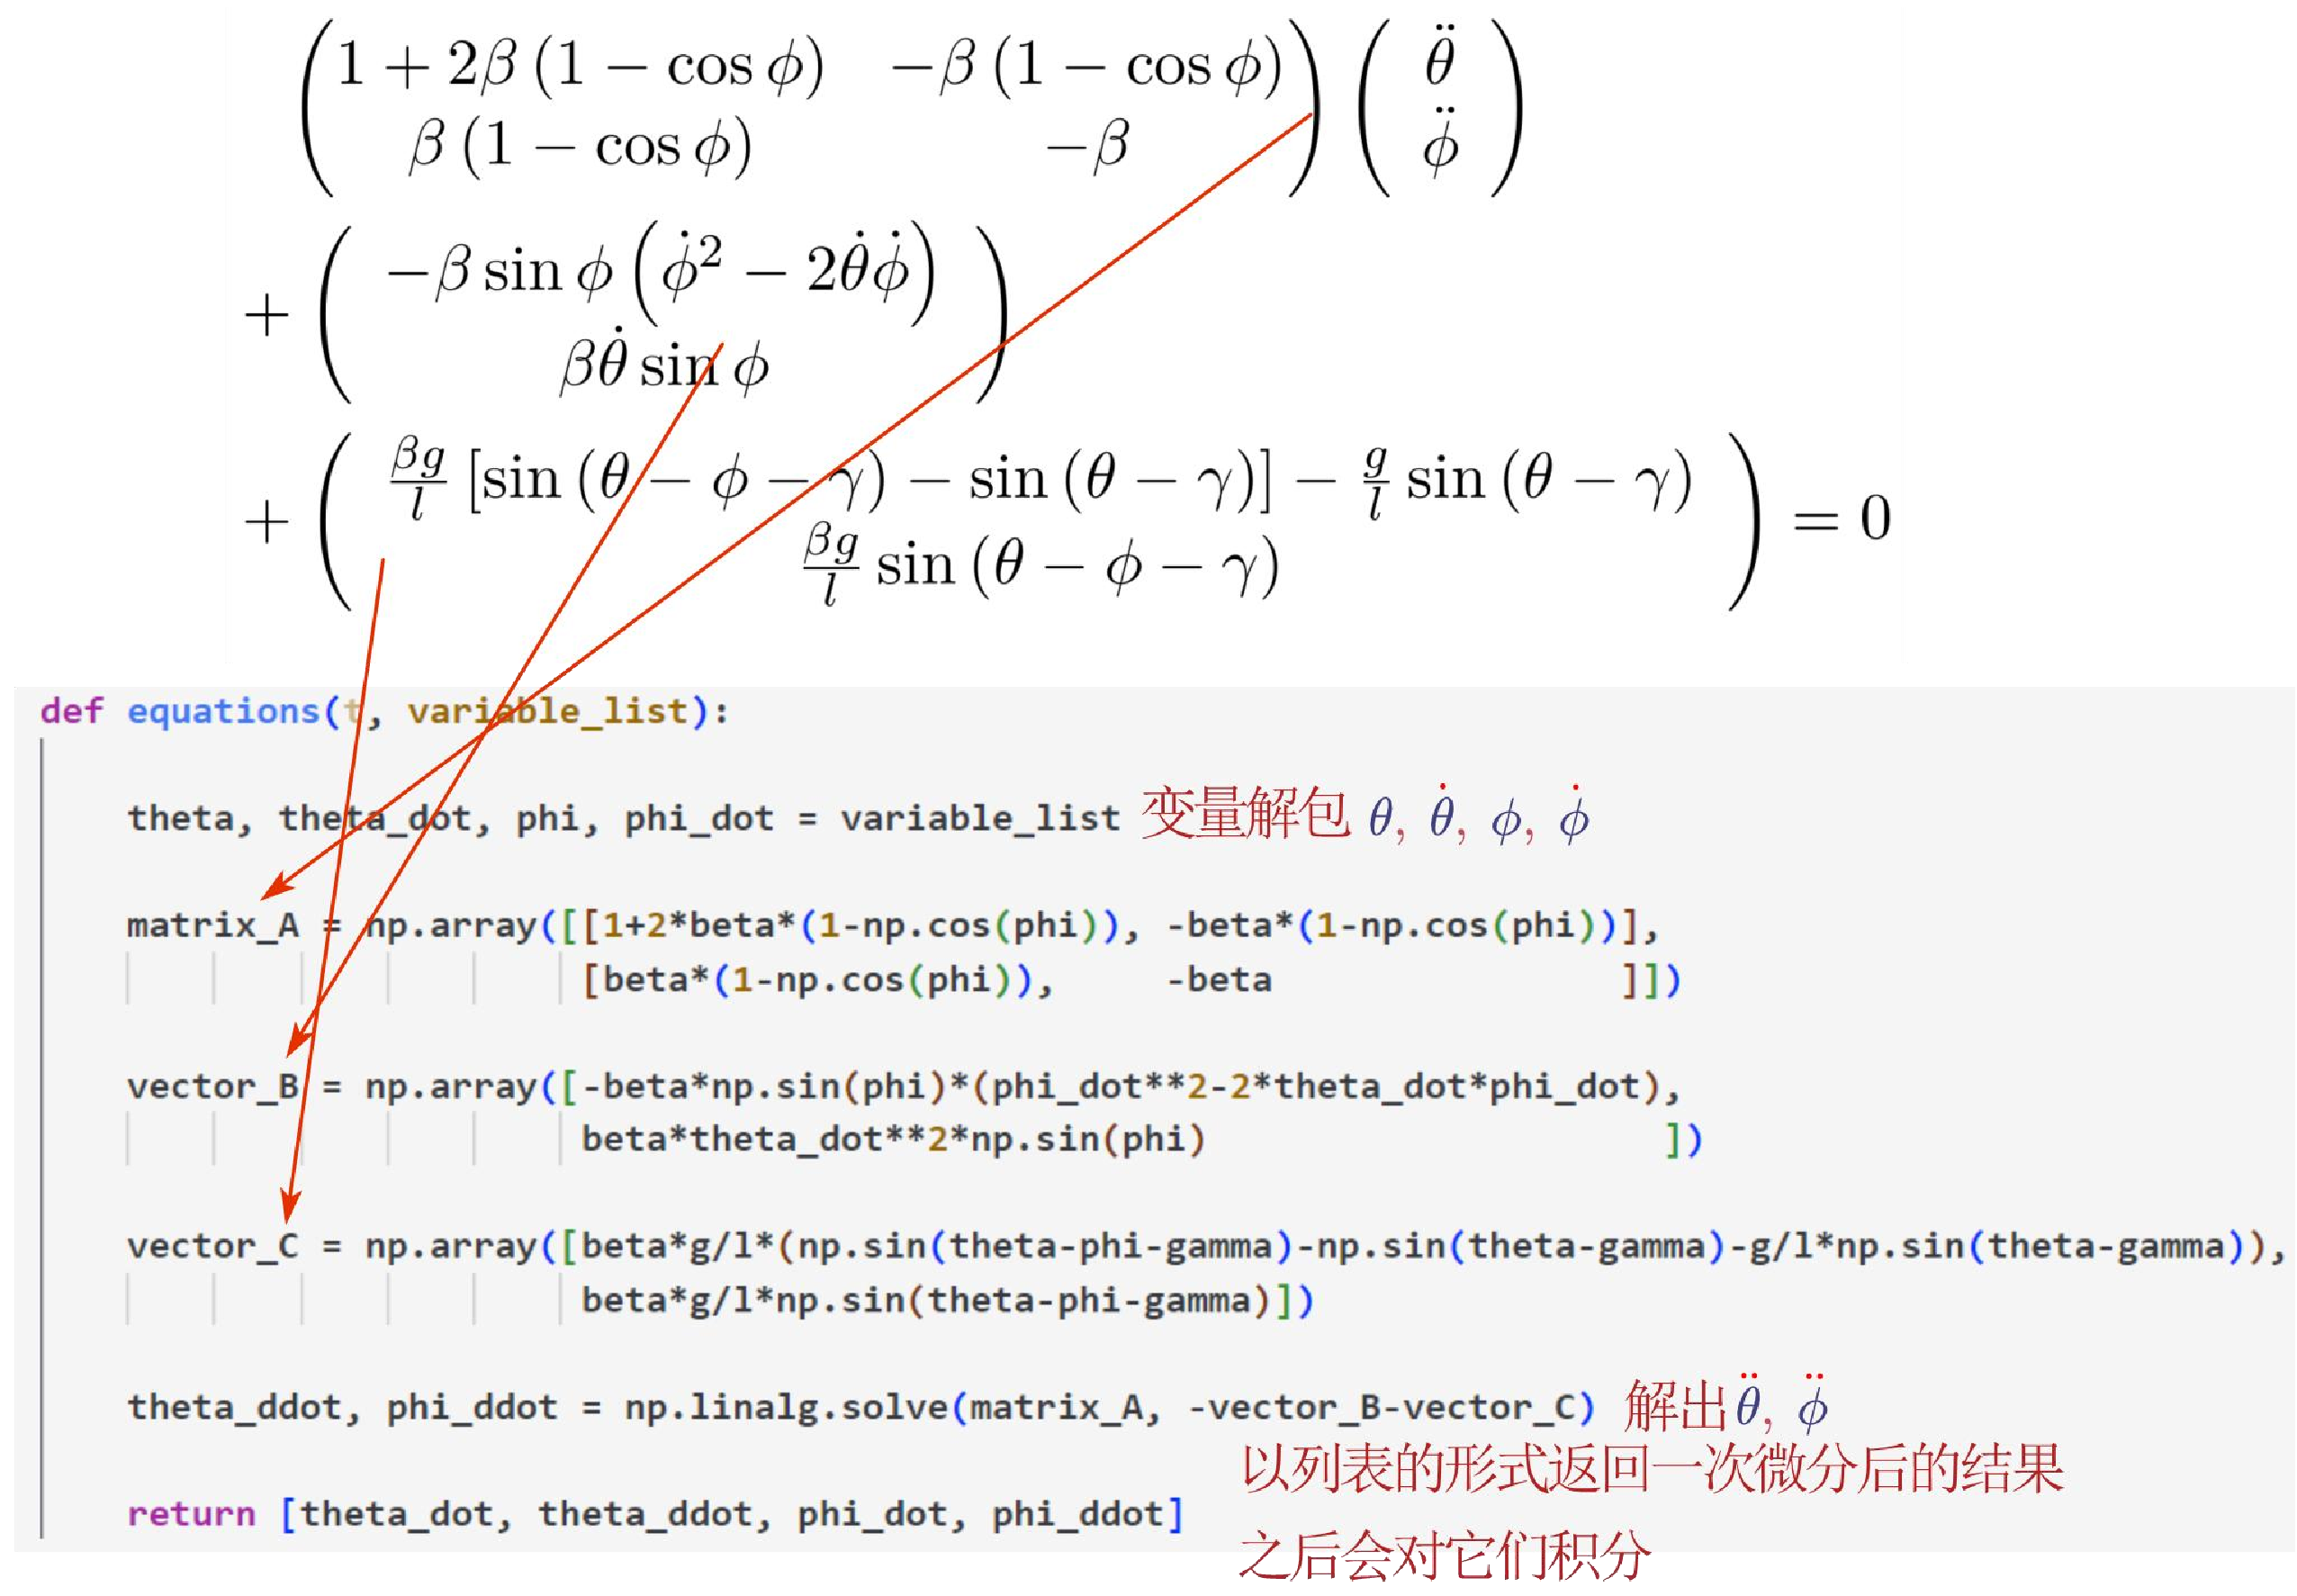
\includegraphics[width=1.1\linewidth]{PythonEquation}
			\caption*{}
			\label{fig:pythonequation}
		\end{figure}
	\end{frame}
	
	\begin{frame}
		\frametitle{定义事件:摆动足触地}
		\begin{figure}
			\centering
			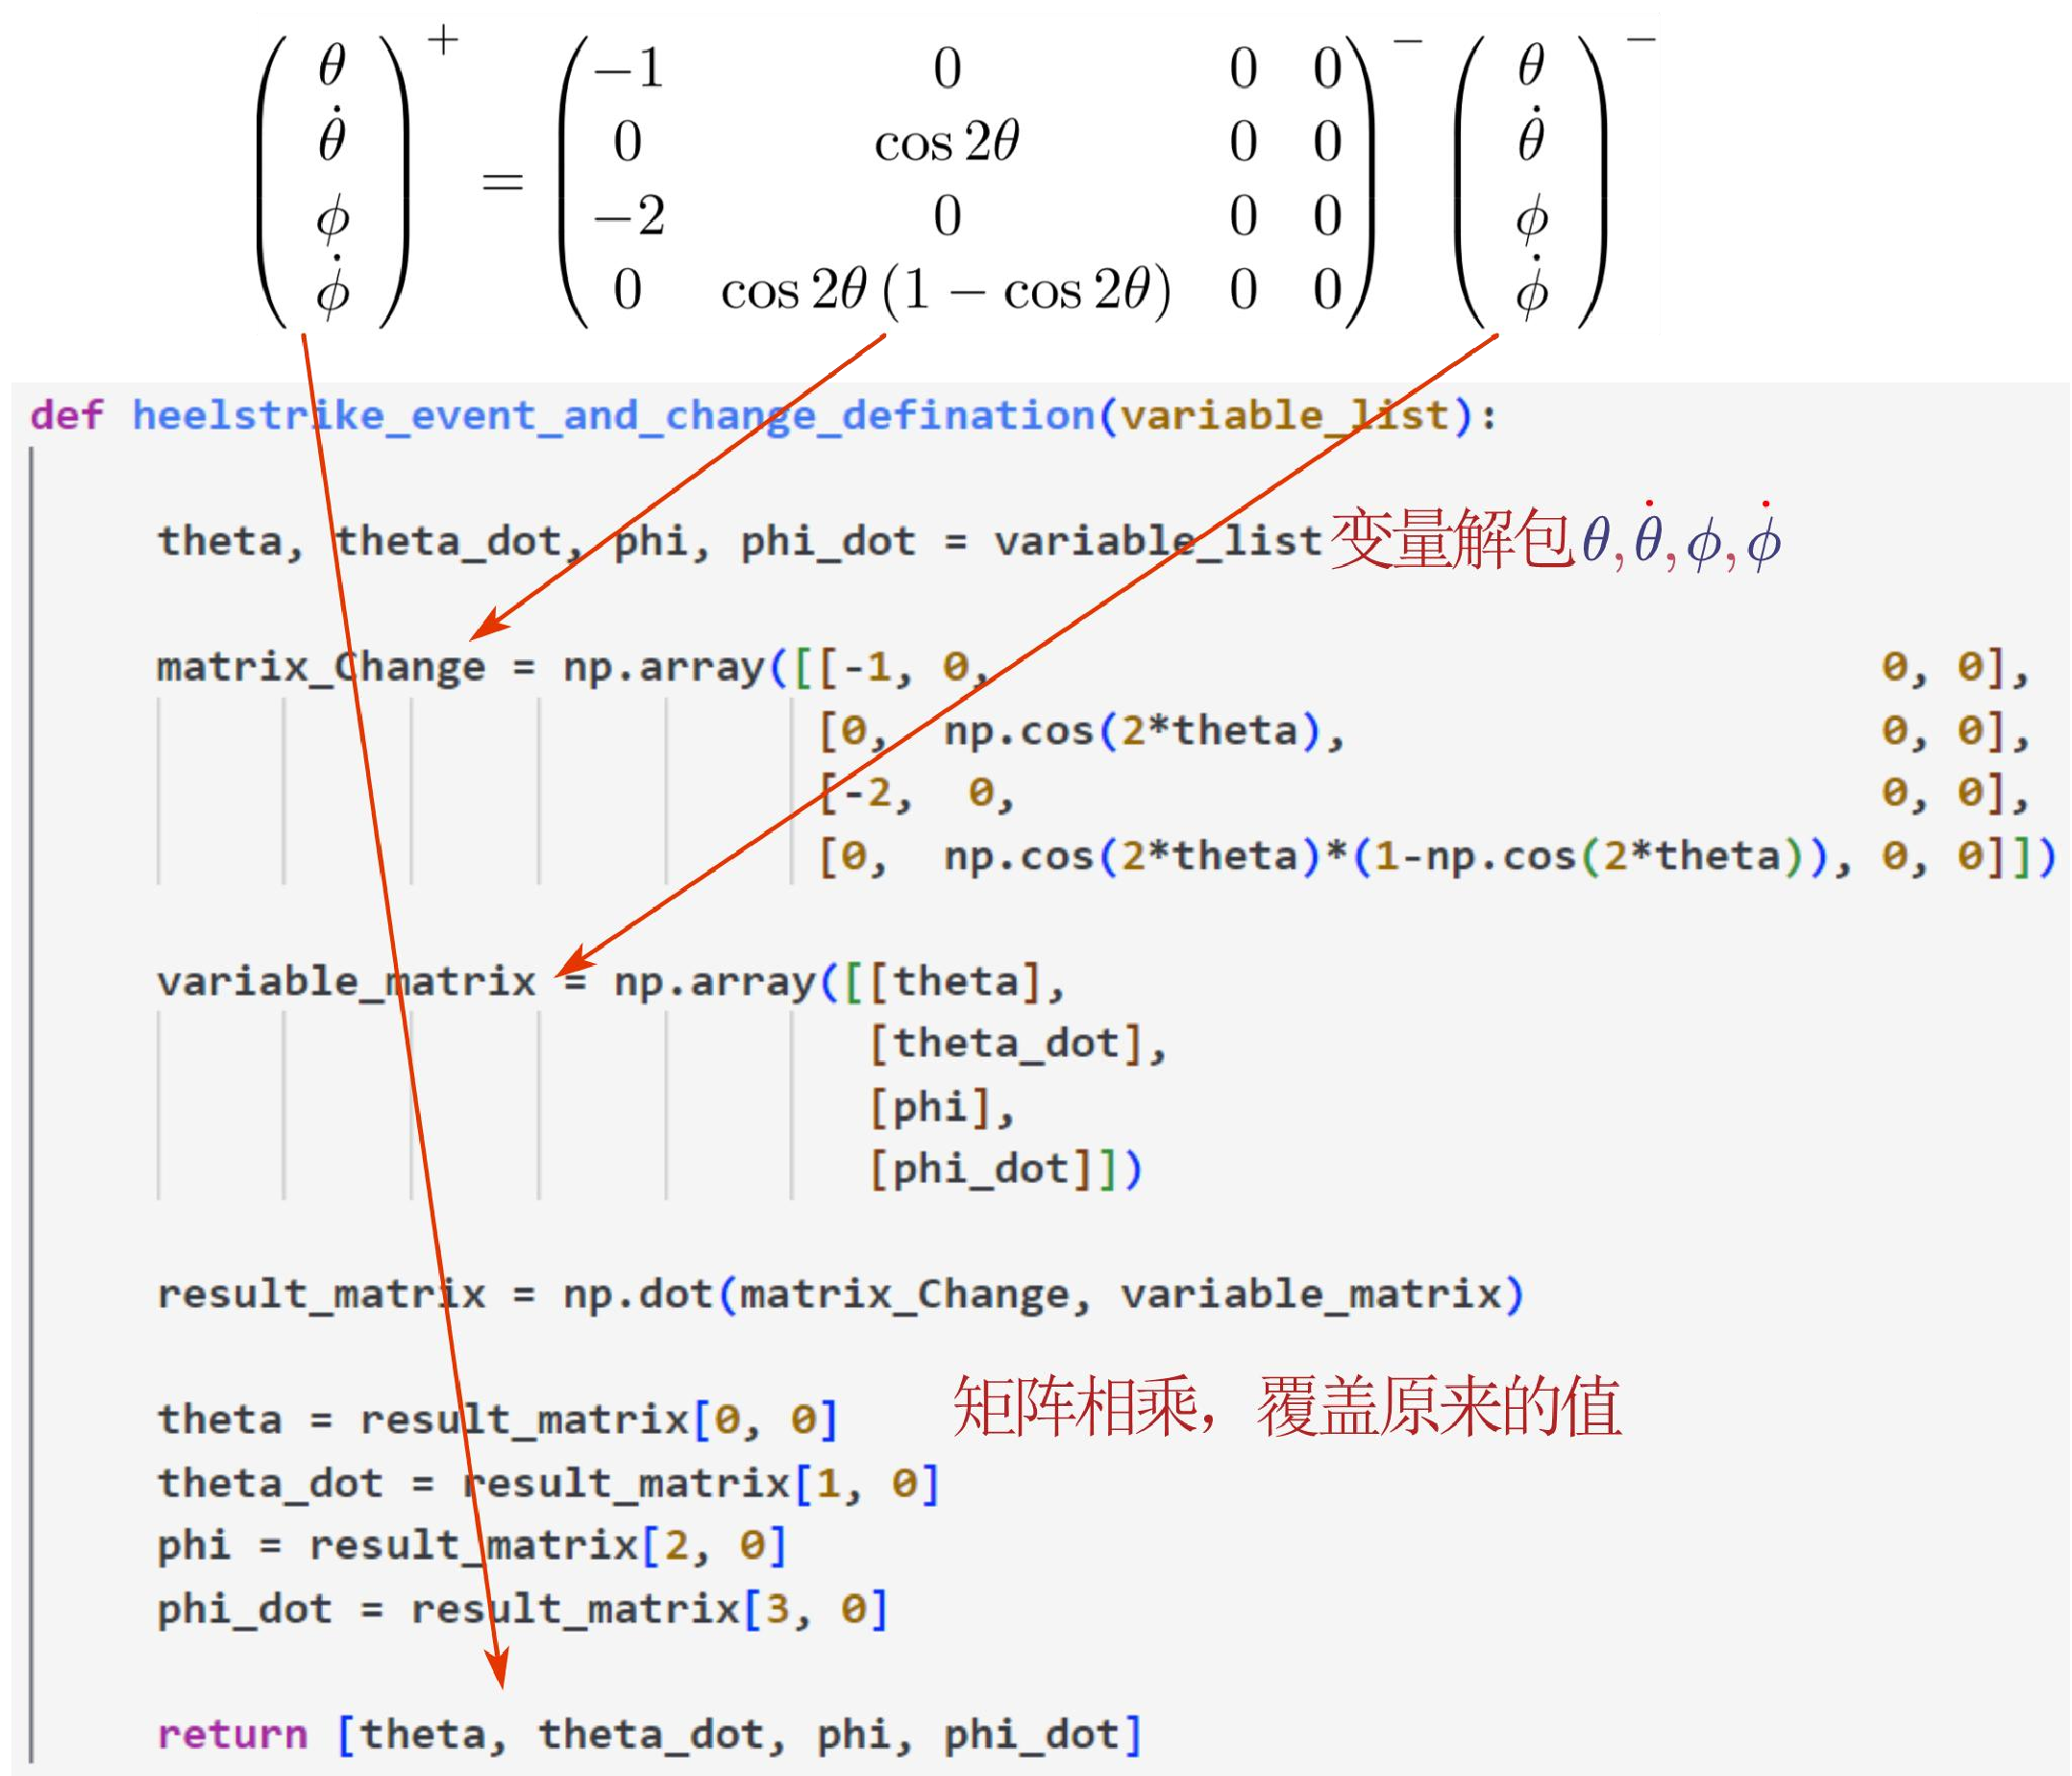
\includegraphics[width=0.9\linewidth]{PythonHeelStrike}
			\caption*{}
			\label{fig:pythonheelstrike}
		\end{figure}
	\end{frame}
	
	\begin{frame}
		\frametitle{事件监测函数}
		\begin{figure}
			\centering
			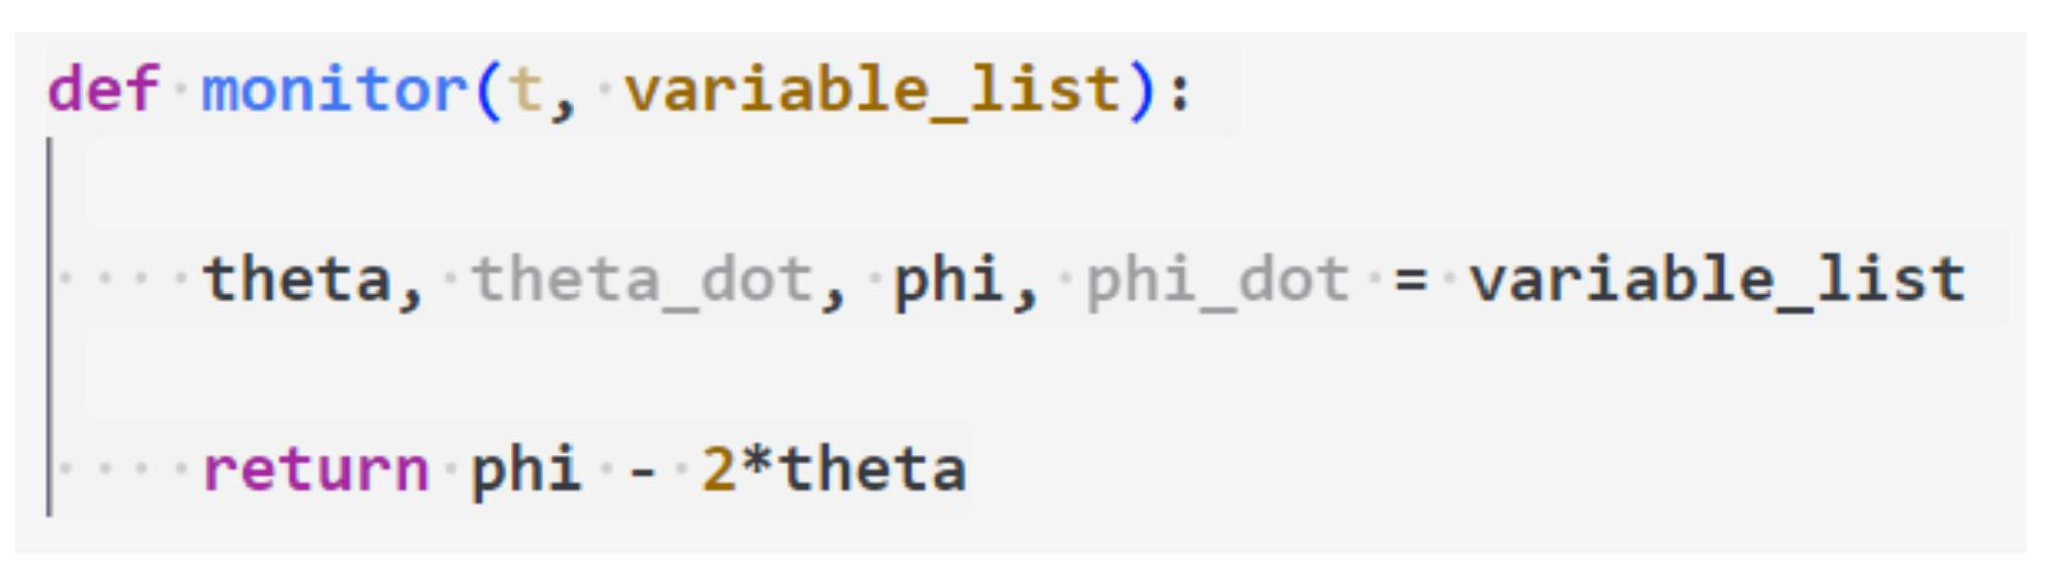
\includegraphics[width=1.0\linewidth]{PythonMonitor}
			\caption*{}
			\label{fig:pythonmonitor}
		\end{figure}
		事件监测函数,监测$\phi-2\theta$的值,当取得0的时候,行走器与斜面构成等腰三角形,也就是说摆动足触地了,触发一次事件
	\end{frame}
	
	\begin{frame}
		\frametitle{循环主体}
		\begin{figure}
			\centering
			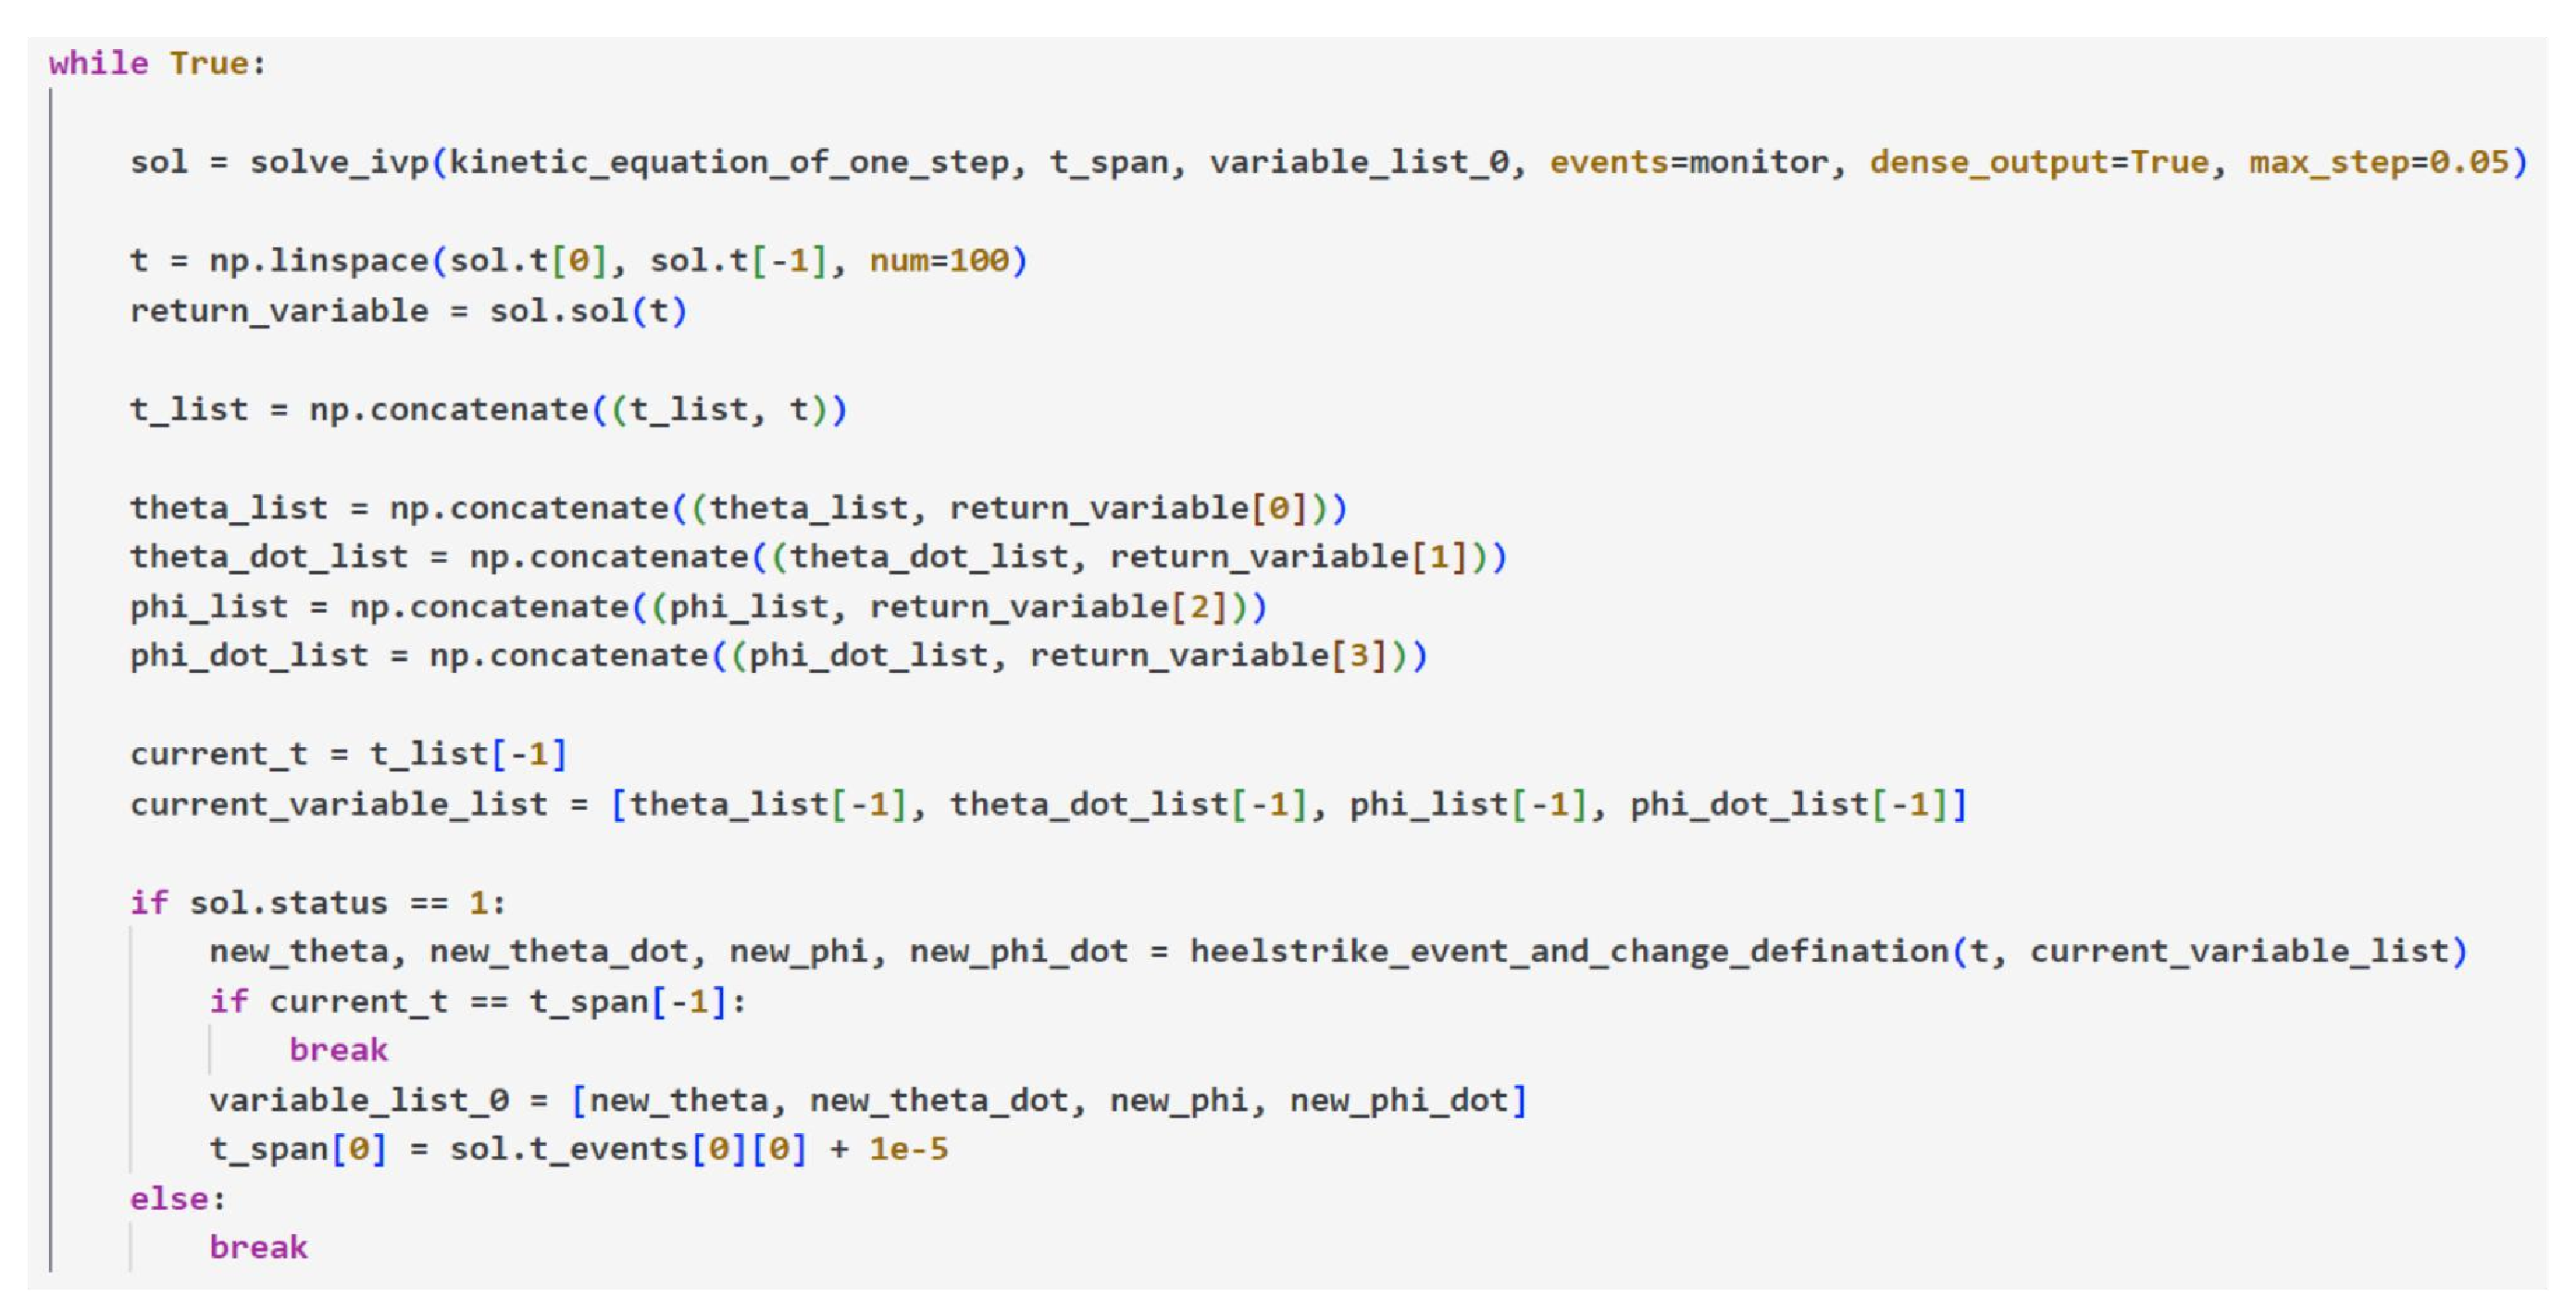
\includegraphics[width=1.1\linewidth]{LoopBody}
			\caption*{}
			\label{fig:loopbody}
		\end{figure}
	\end{frame}
	
	\begin{frame}
		\frametitle{结果}
		\begin{figure}
			\centering
			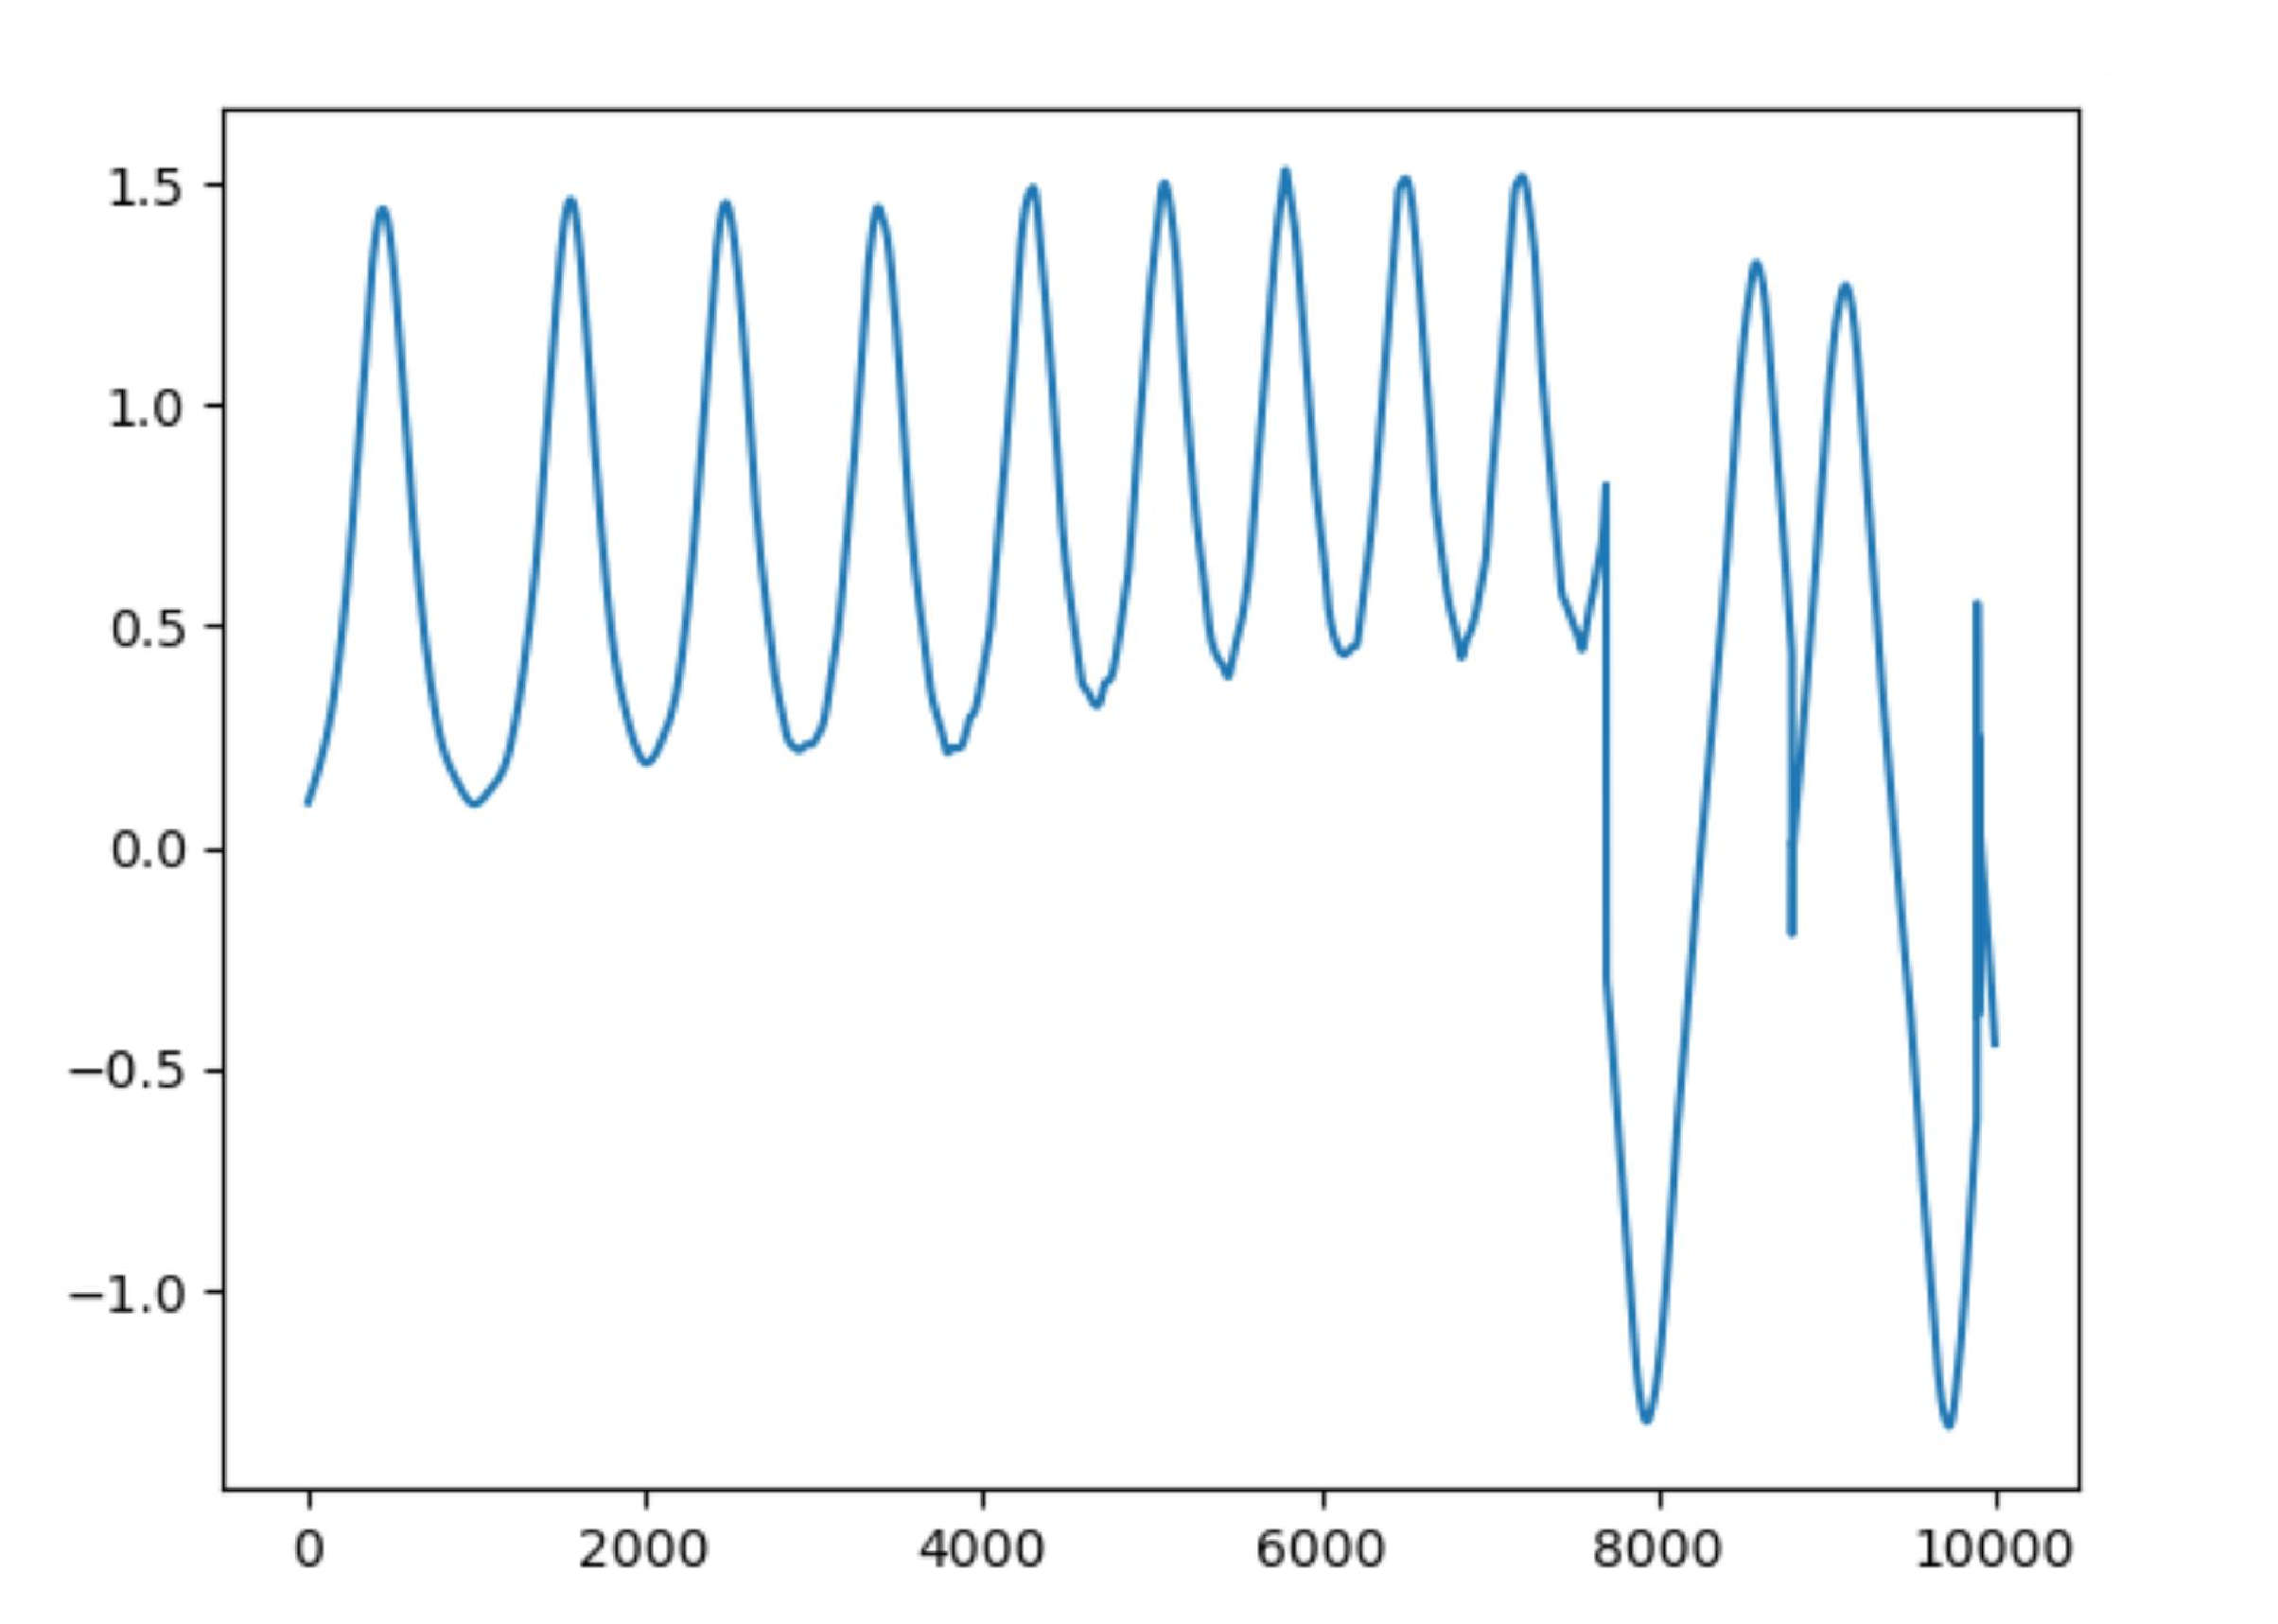
\includegraphics[width=0.8\linewidth]{Result}
			\caption*{}
			\label{fig:result}
		\end{figure}
		效果不是特别好,突变不明显(过于光滑),解不稳定
	\end{frame}
	
	\begin{frame}
		\frametitle{后续的改进思路}
		\begin{enumerate}
			\item 一个直接的原因是参数设置不当,由于原论文没有详细给出模拟实验参数(初始的角度,速度),所以需要自己摸索
			\item 求解器刚性处理不足,需要改进代码
			\item \textbf{如何迁移这种做法到四足复杂模型中?对于这种简单模型,数值计算都无法令人满意,如何进行复杂模型的运算?}
		\end{enumerate}
	\end{frame}
	%%%%%%%%%%%%%%%%%%%%%%%%%%%%%%%%%%%%%%%%%%%%%%%%%%%%%%%%%%%%%%%%%%%%%%%%%%%%%%%%%%%%%%%%%%%%%%%	
	
	%参考文献(非调用.bib文件,而是手动输入)
	%举例:Jones, Edward. 2020. "Studies in Grass Biology." Journal of Plant Research 15 (2): 123-145. https://doi.org/10.1086/123456.
	
	% Lastname, Firstname. Year. "Article Title." Journal Name volume (issue): page range. DOI or URL.
	
	\appendix
	\begin{frame}{参考文献}
		\begin{thebibliography}{99} % 最大可能的参考文献编号宽度,可以根据实际情况调整
			\bibitem[Author et al., 2021]{ref1}
			[1]Garcia, Mariano, Anindya Chatterjee, Andy Ruina, and Michael Coleman. 1998. "The Simplest Walking Model: Stability, Complexity, and Scaling." ASME Journal of Biomechanical Engineering. Accepted April 16, 1997; final version February 10, 1998.
			\bibitem[Author et a2., 2024]{ref2}
			[2]感谢\,谢昀城\,学长的在代码改进方面指导
		\end{thebibliography}
	\end{frame}
	
	\begin{frame}[plain,c]
		\begin{center}
			\Huge END
		\end{center}
	\end{frame}
	
\end{document}